\chapter{头颈部}

\section{正常X线解剖}

\begin{figure}[!htbp]
 \centering
 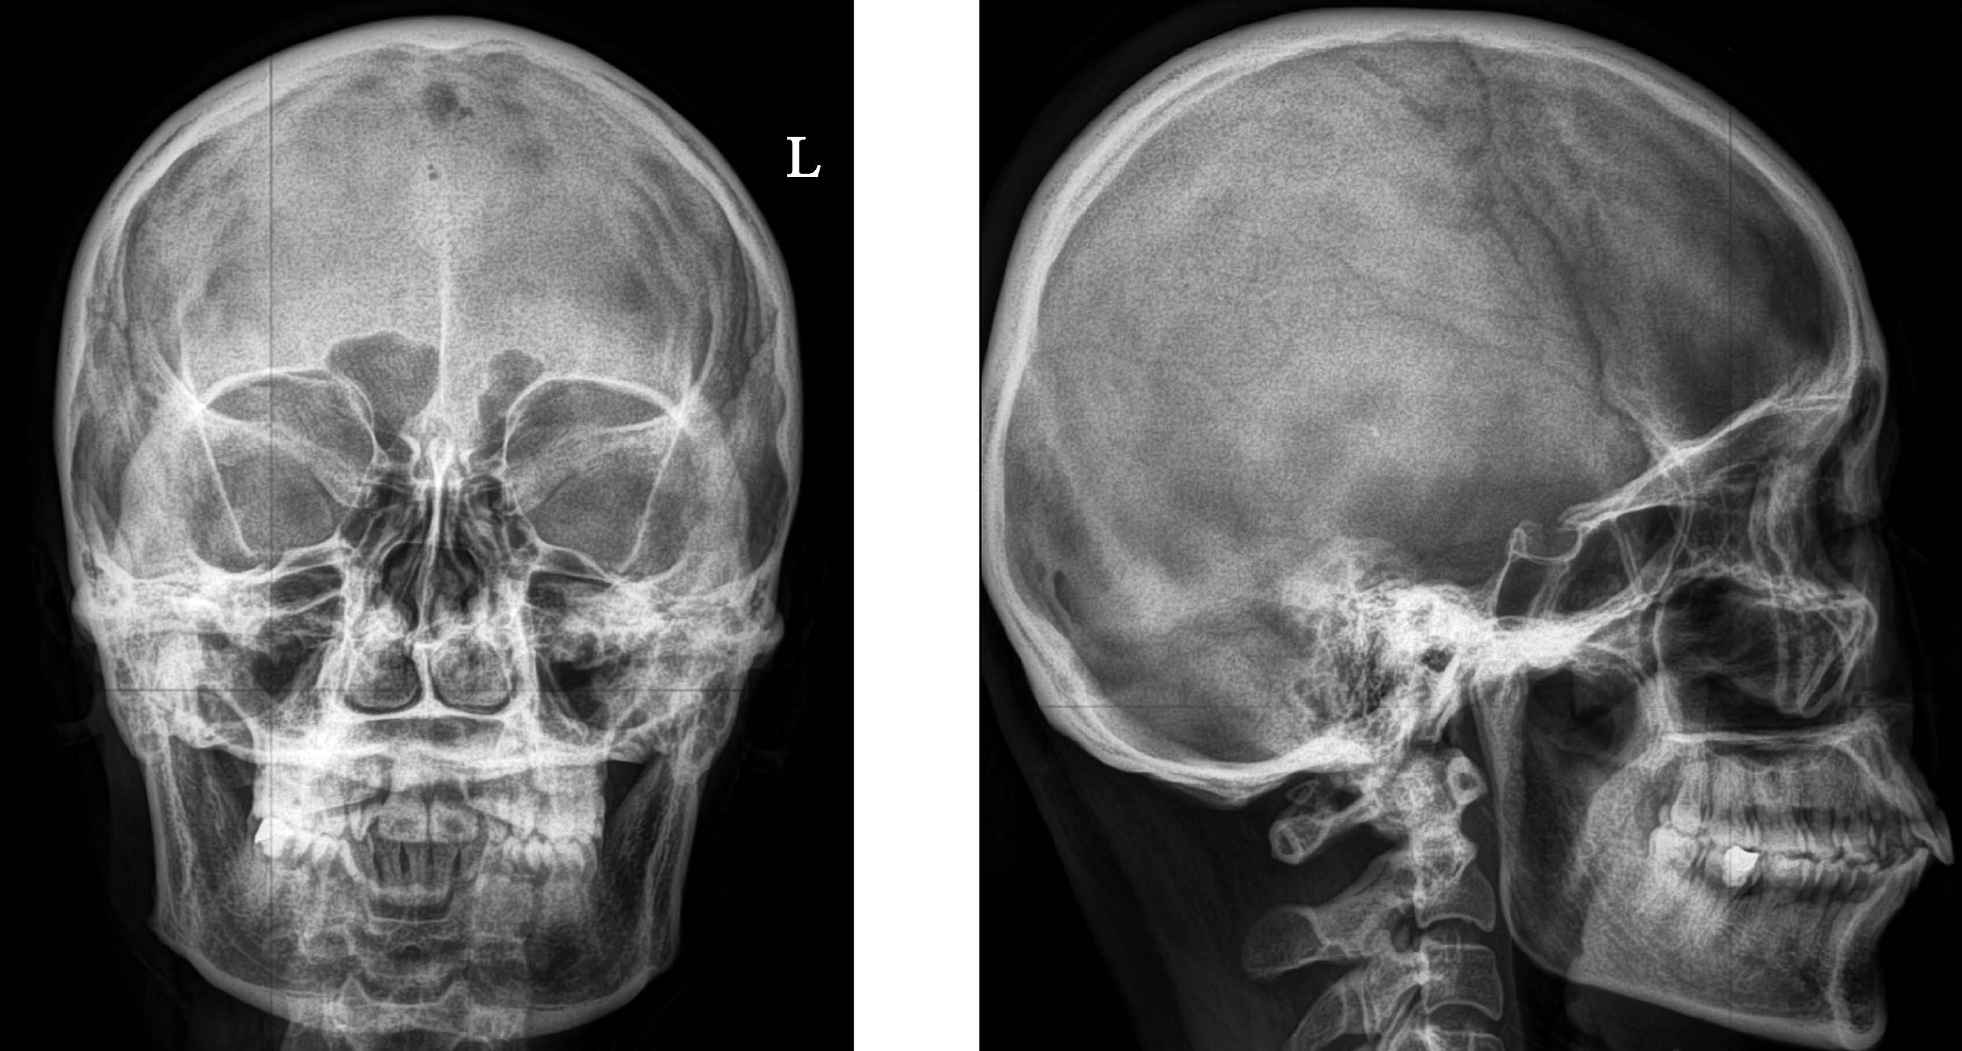
\includegraphics{./images/Image00411.jpg}
 \captionsetup{justification=centering}
 \caption{正常眼眶正位片和侧位片}
 \label{fig7-1-1}
  \end{figure} 

\textbf{【X线表现】}
 两侧眼眶对称,骨质连续光滑,眶内密度正常,未见明显占位影,眶上裂基本对称。

\textbf{【X线诊断】}  正常眼眶。

\begin{figure}[!htbp]
 \centering
 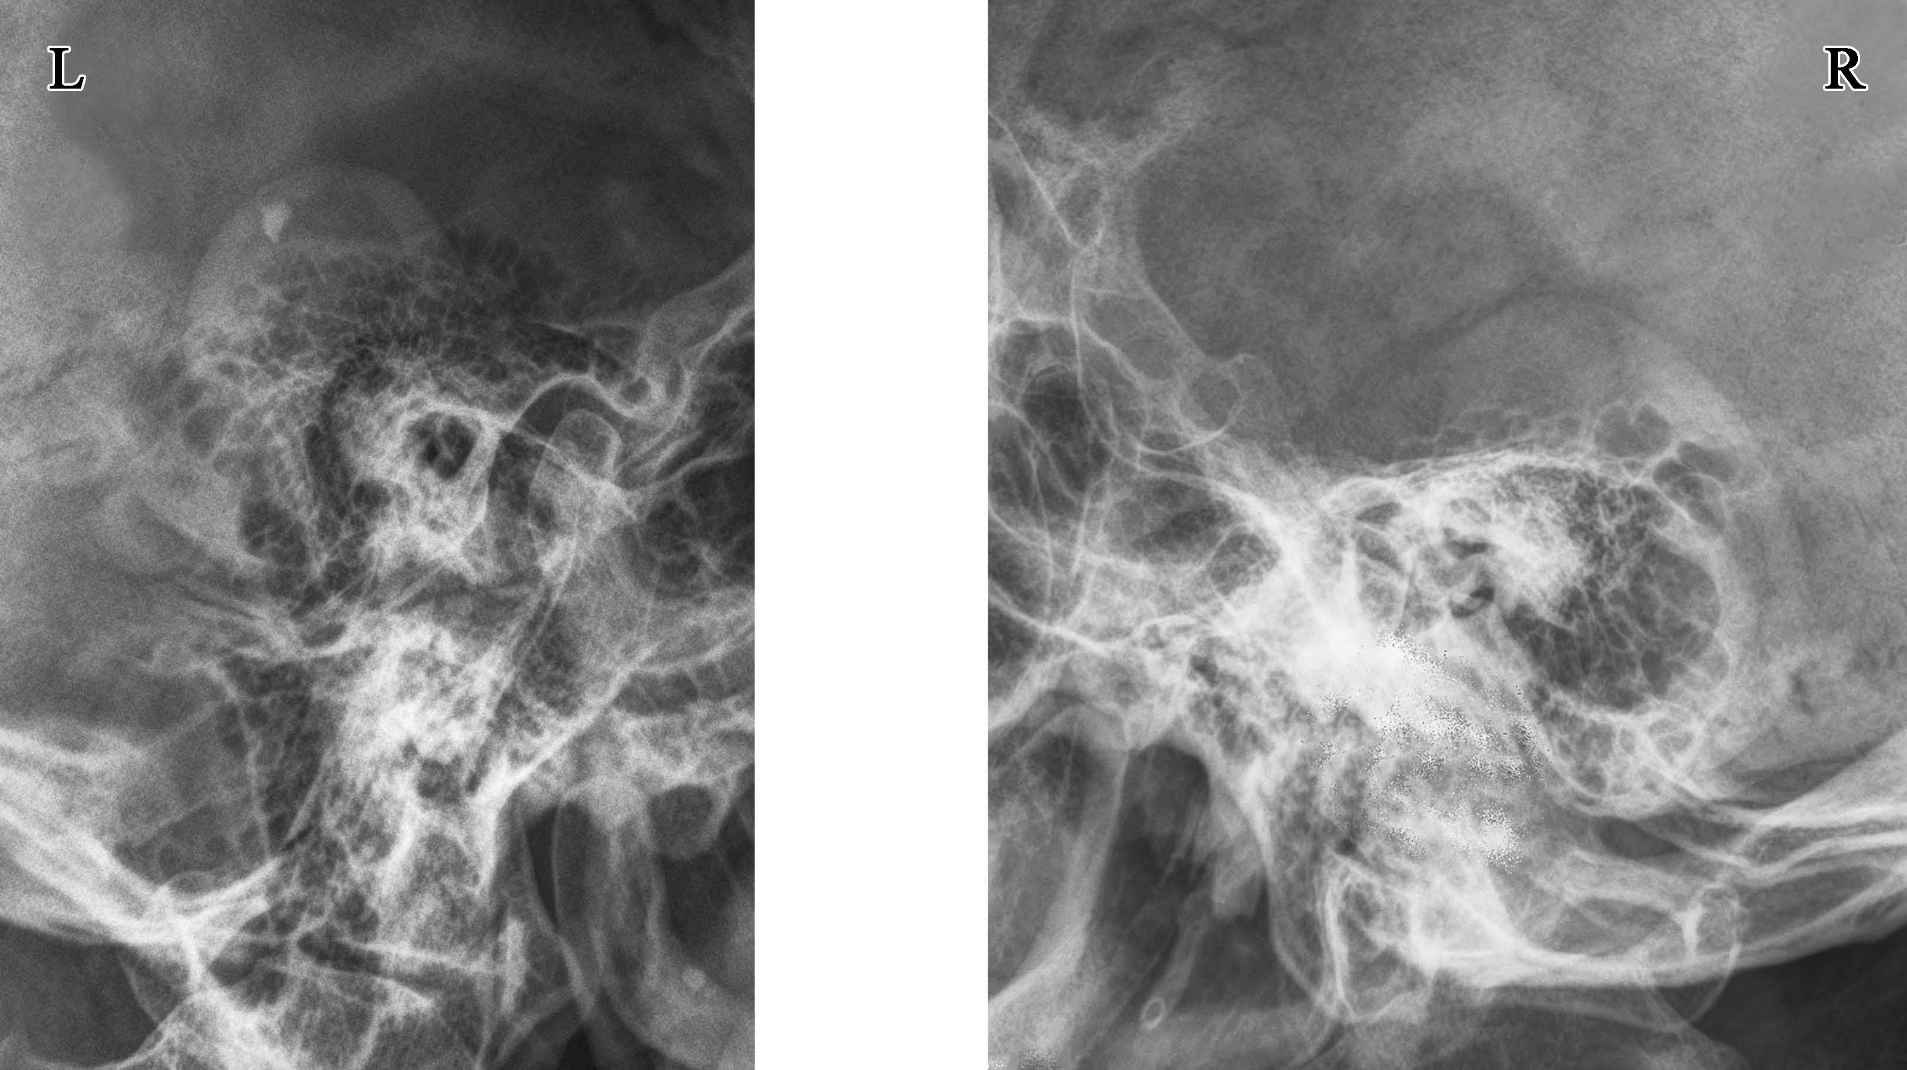
\includegraphics{./images/Image00412.jpg}
 \captionsetup{justification=centering}
 \caption{左、右乳突梅氏位}
 \label{fig7-1-2}
  \end{figure} 

\textbf{【X线表现】}
 双侧乳突气化良好,气房集中在鼓窦周围,气房向周边发展,容积逐渐变大,呈扇样分布。气房骨间隔由大小不等的致密骨组成,呈蜂窝状。

\textbf{【X线诊断】}  正常乳突梅氏位。

\begin{figure}[!htbp]
 \centering
 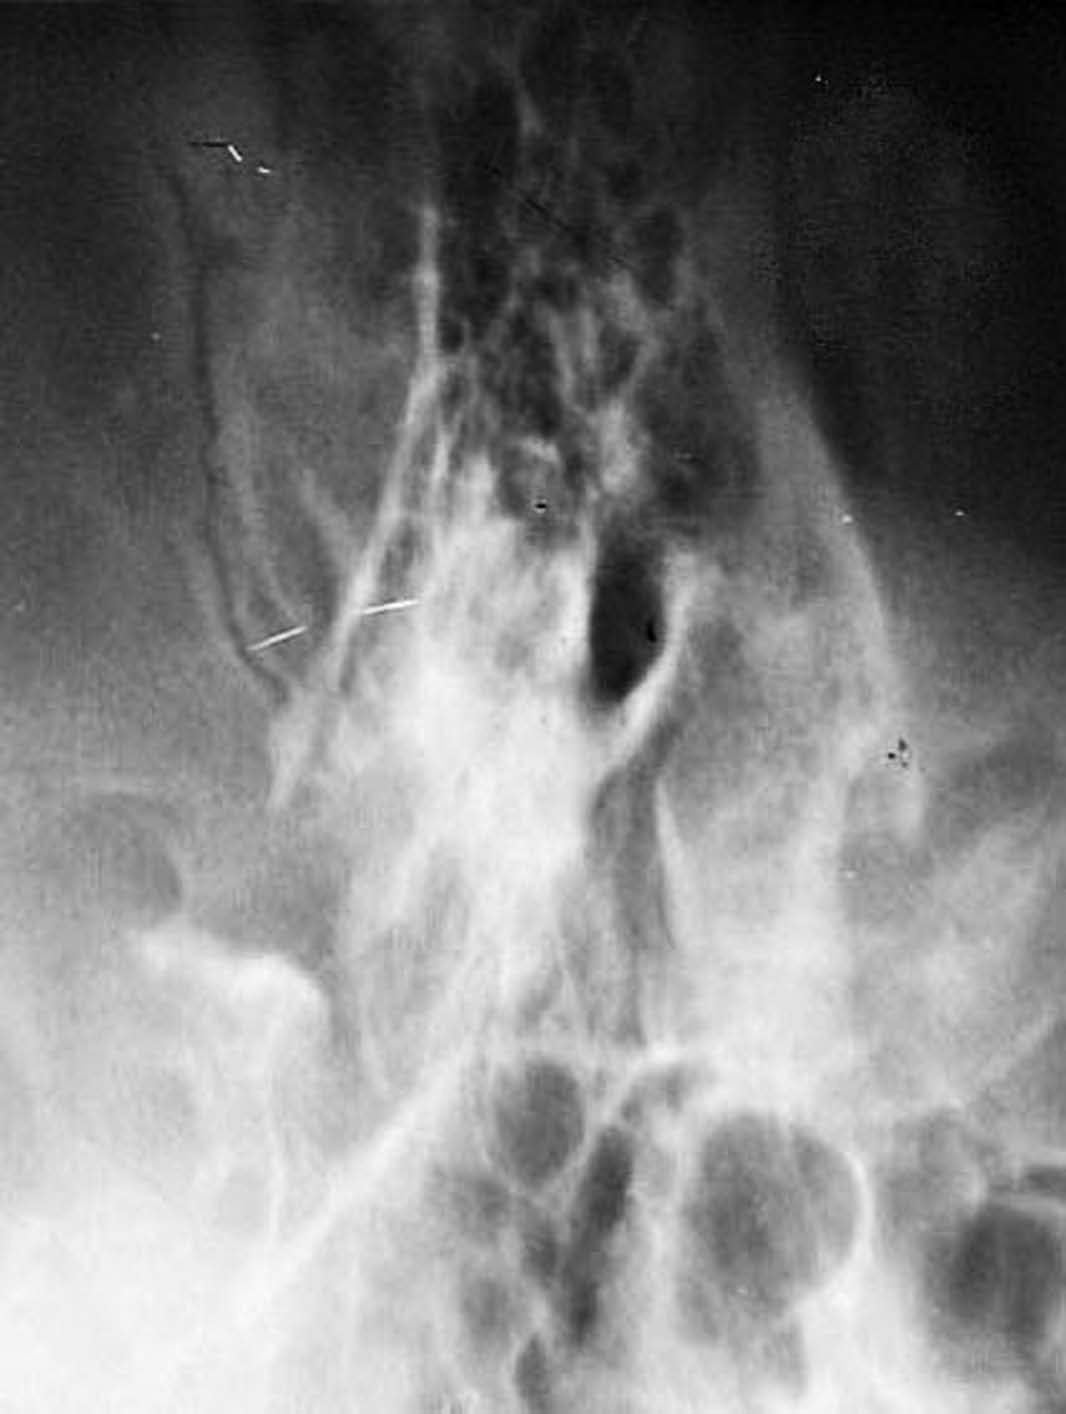
\includegraphics{./images/Image00413.jpg}
 \captionsetup{justification=centering}
 \caption{右侧乳突梅氏位}
 \label{fig7-1-3}
  \end{figure} 

\textbf{【X线表现】}
 外耳孔位于正中,上鼓室、鼓窦及鼓室入口可清晰显示。骨质连续,未见破坏。

\textbf{【X线诊断】}  正常气化型乳突。

\begin{figure}[!htbp]
 \centering
 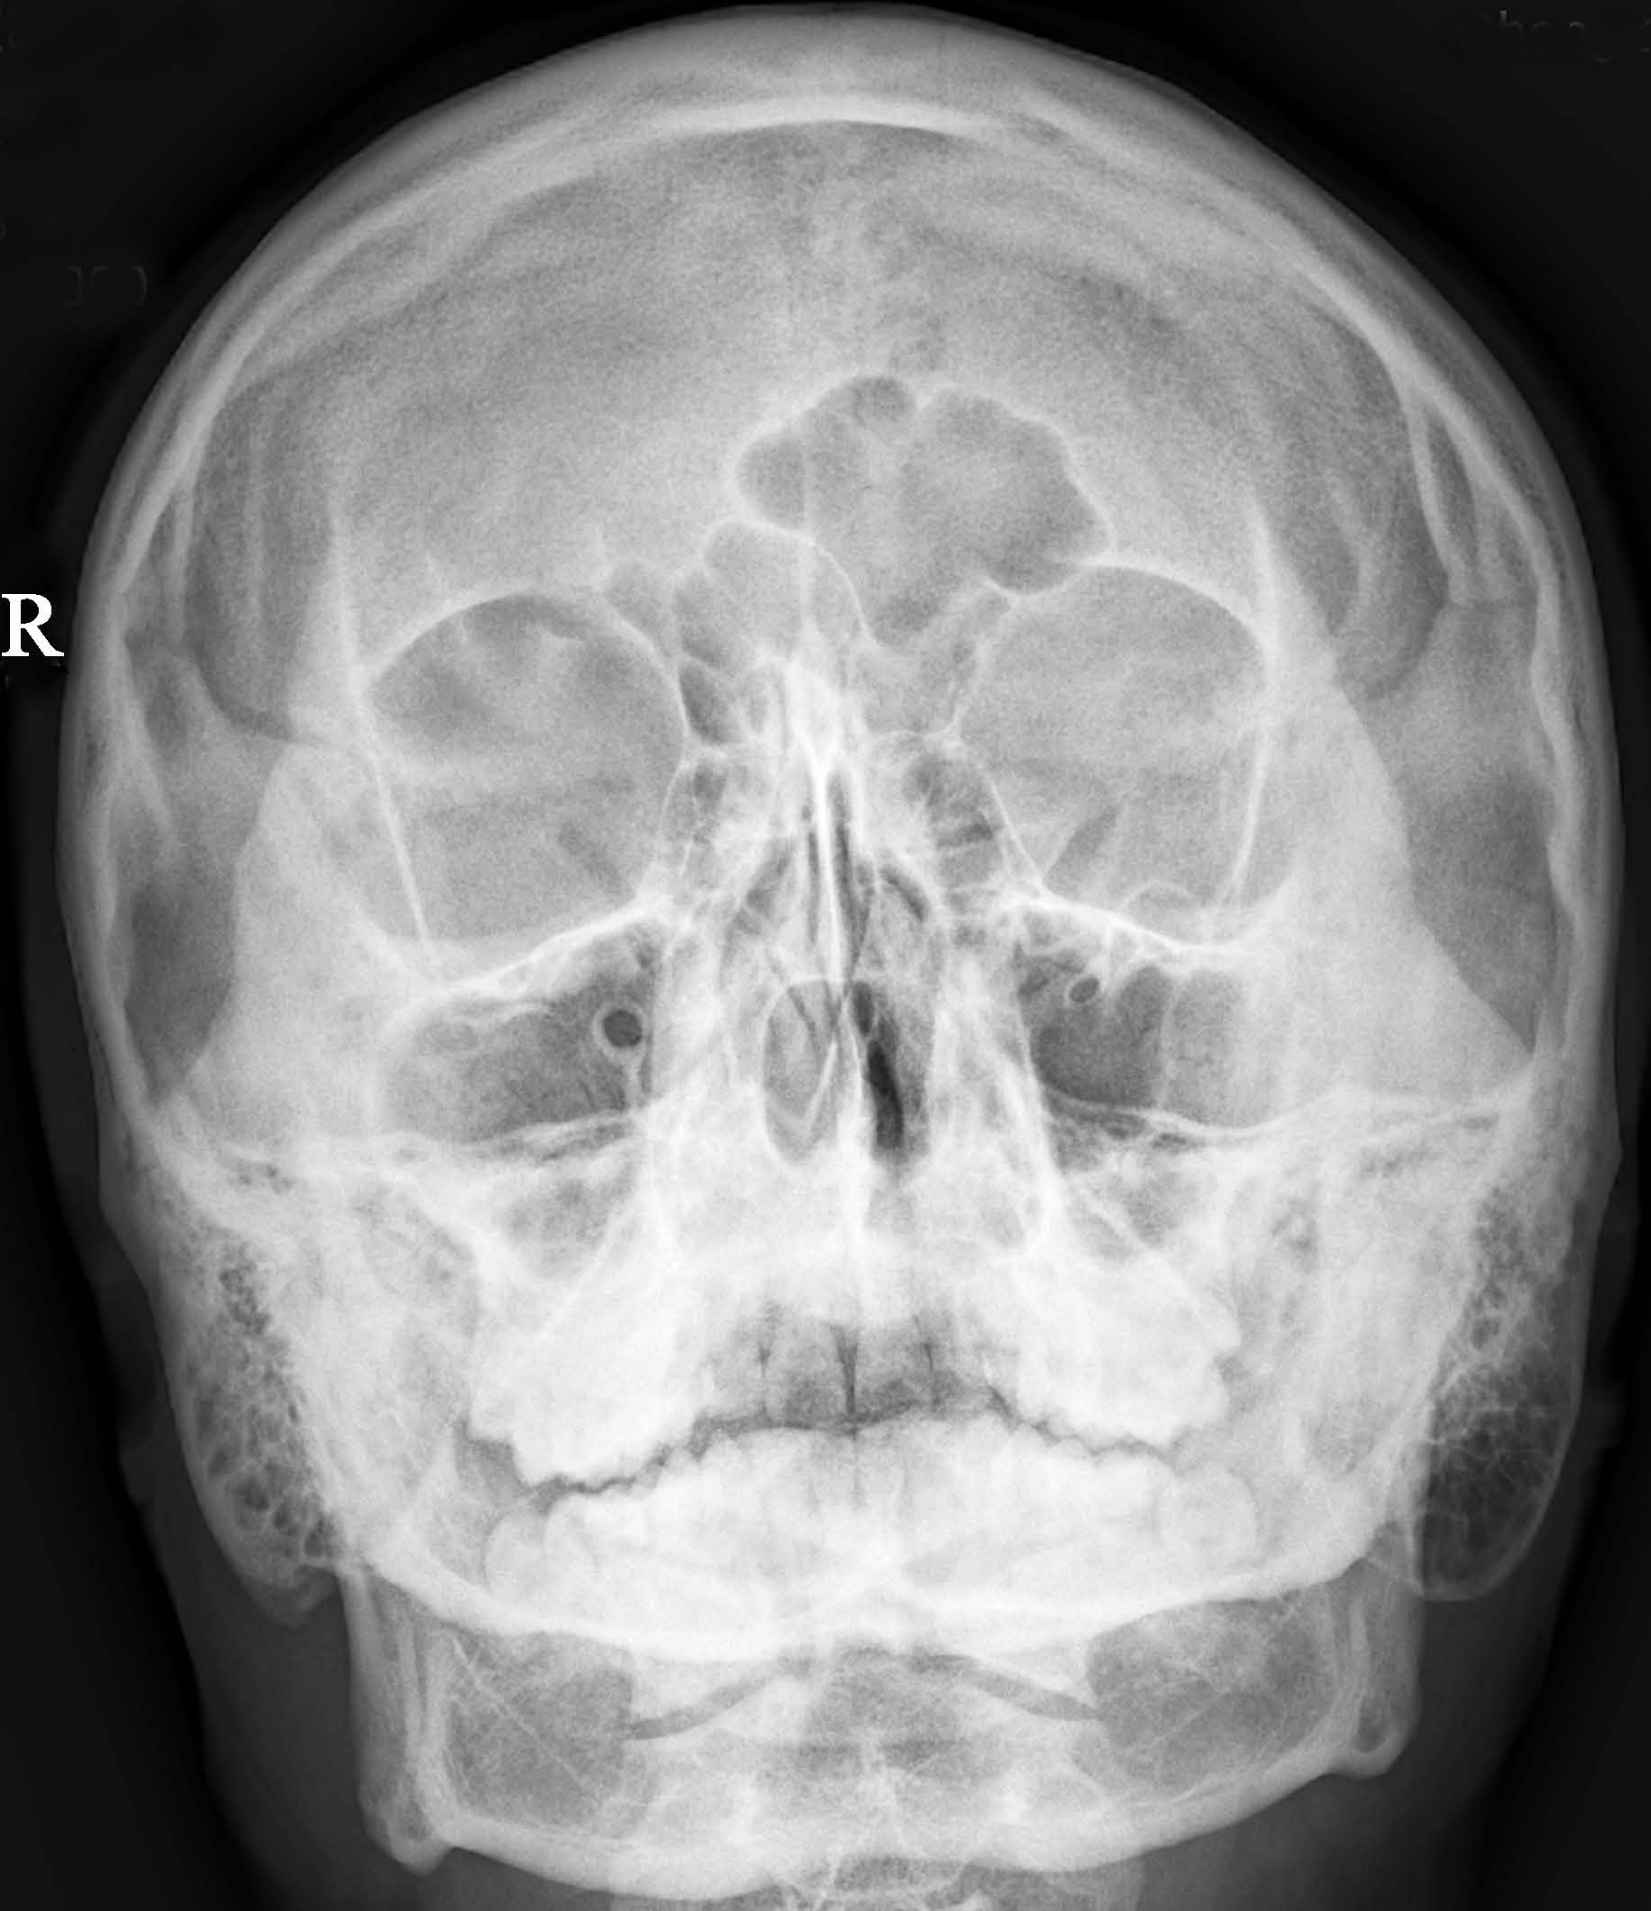
\includegraphics{./images/Image00414.jpg}
 \captionsetup{justification=centering}
 \caption{鼻旁窦华氏位}
 \label{fig7-1-4}
  \end{figure} 

\textbf{【X线表现】}
 显示双侧鼻旁窦包括上颌窦、筛窦及额窦窦壁光整,未见破坏,窦腔清晰呈低密度,未见软组织影。与双侧眼眶密度接近。

\textbf{【X线诊断】}  正常鼻旁窦华氏位。

\textbf{【评  述】}
 为检查鼻旁窦常规应用的位置,可分为坐位及卧位。坐位对观察上颌窦内有无积液较好。

\begin{figure}[!htbp]
 \centering
 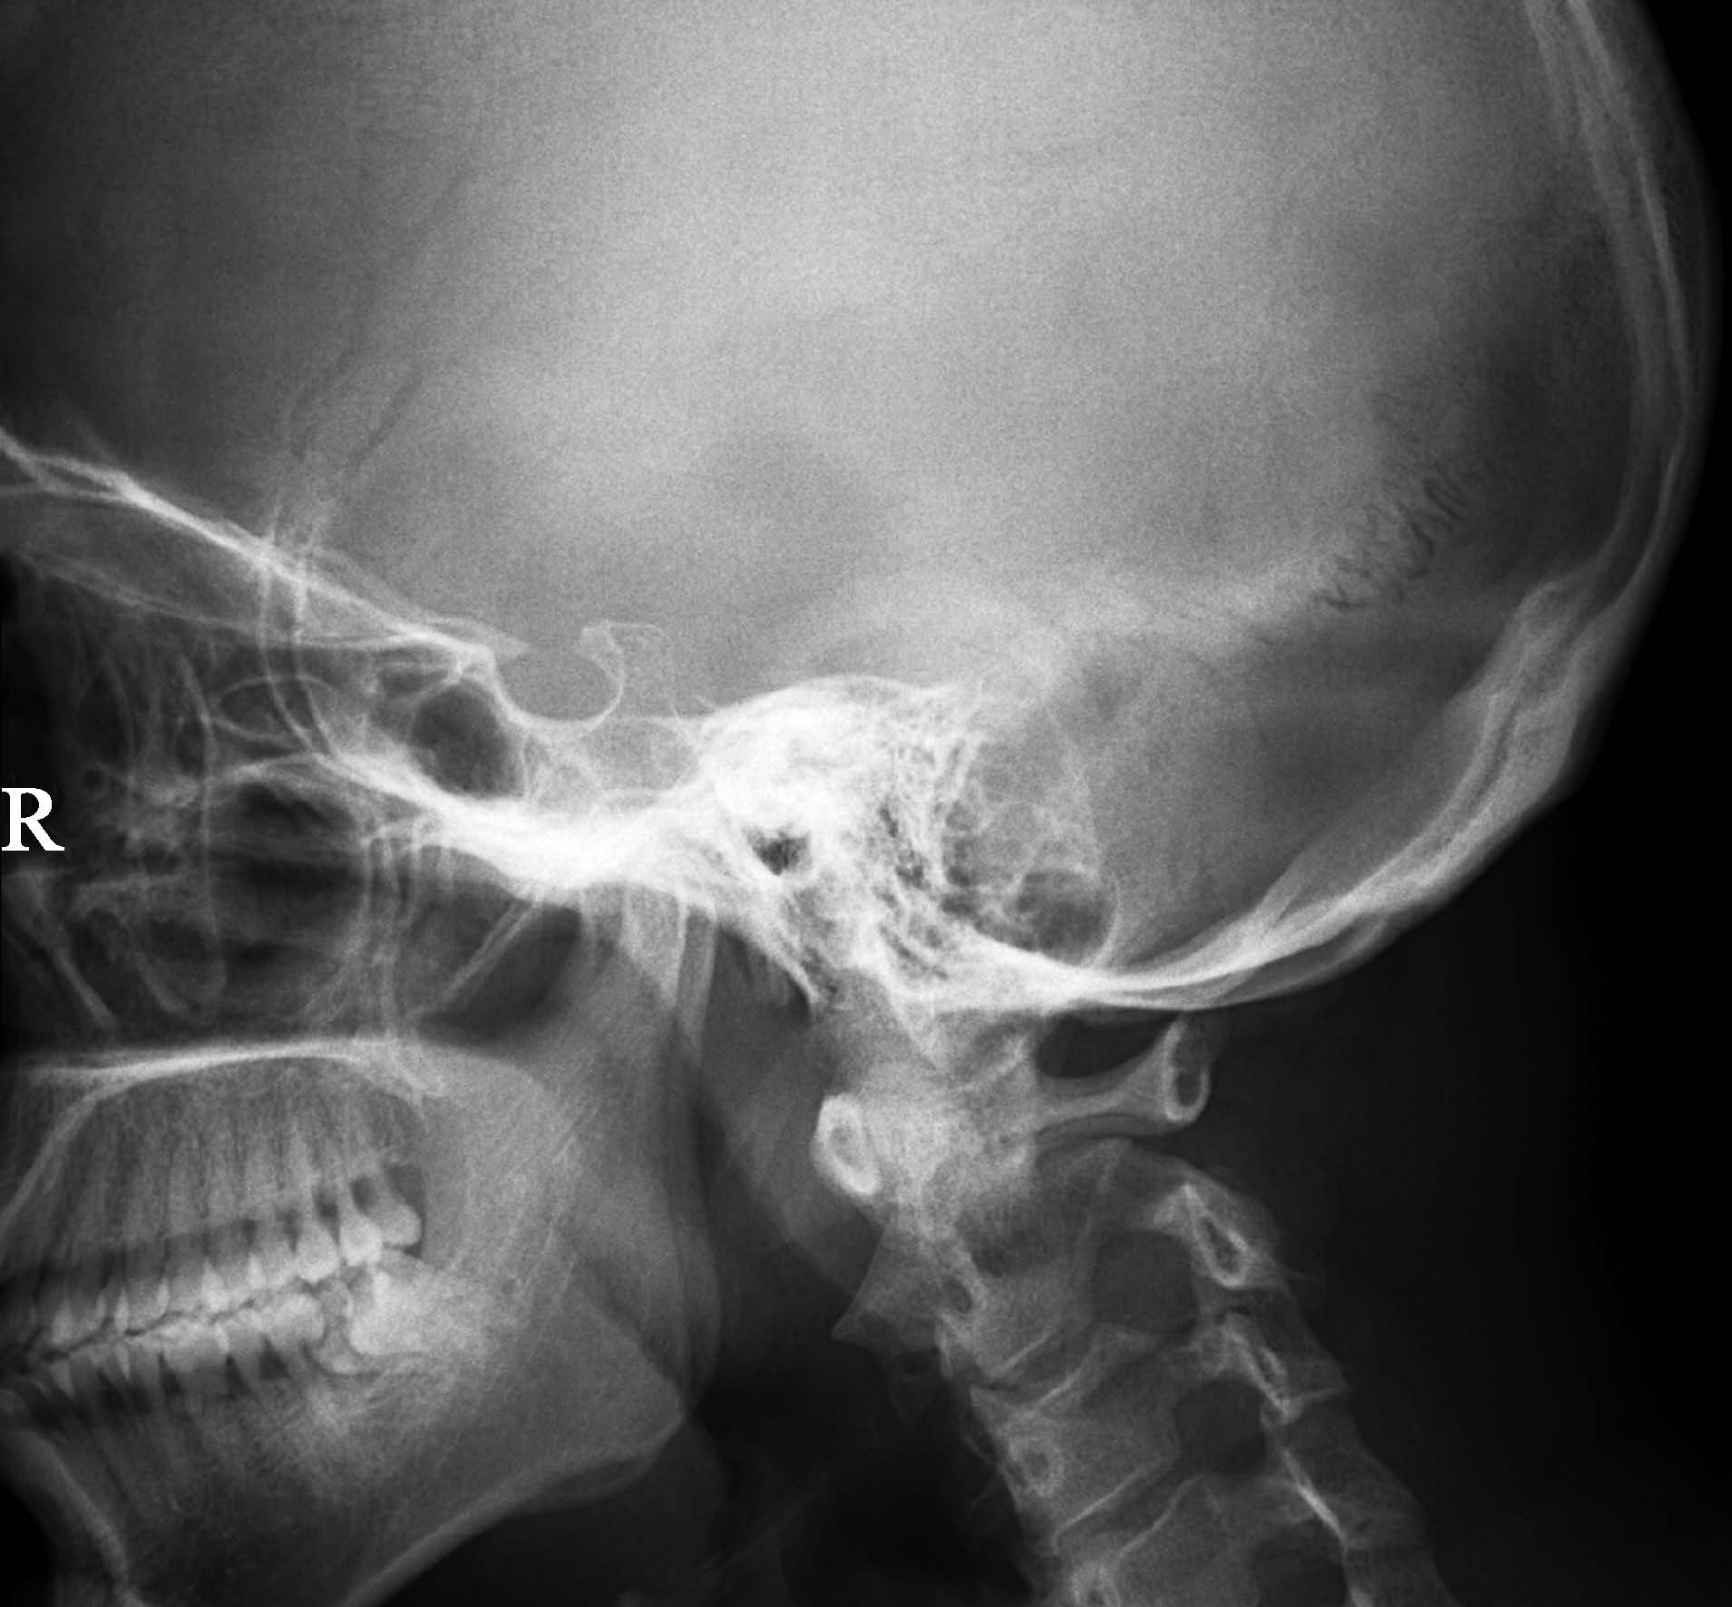
\includegraphics{./images/Image00415.jpg}
 \captionsetup{justification=centering}
 \caption{蝶窦侧位片}
 \label{fig7-1-5}
  \end{figure} 

\textbf{【X线表现】}
 蝶窦位于蝶骨体中央,气化良好,鞍结节及鞍背显示较清楚,垂体窝位于正中,其内垂体密度正常,未见异常密度影。

\textbf{【X线诊断】}  正常蝶窦。

\begin{figure}[!htbp]
 \centering
 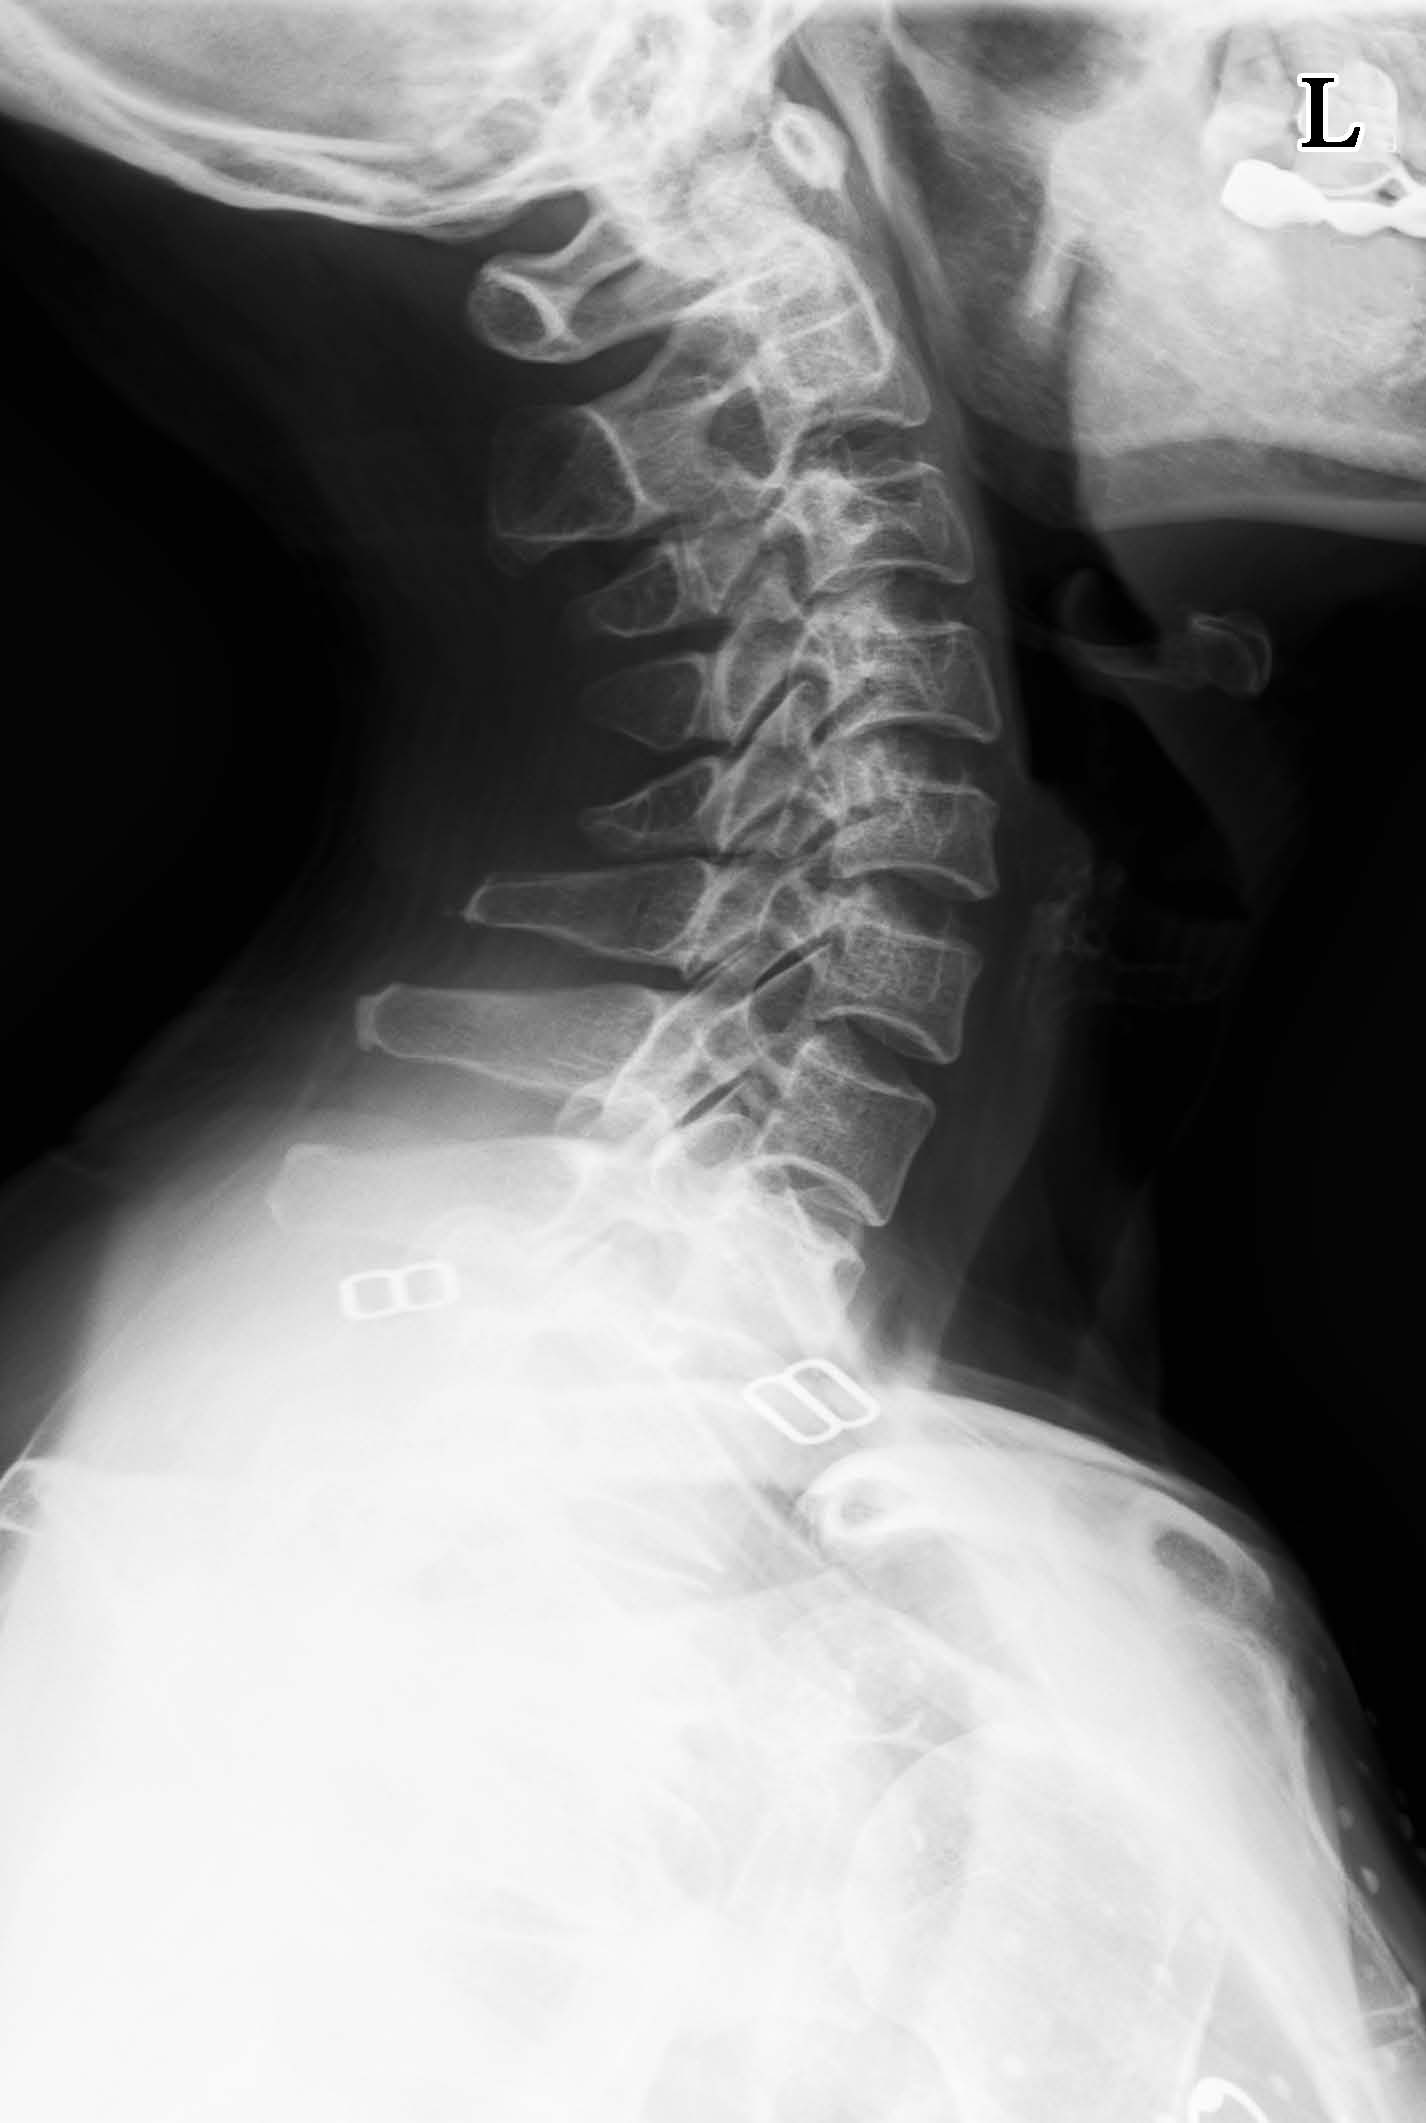
\includegraphics{./images/Image00416.jpg}
 \captionsetup{justification=centering}
 \caption{颈部侧位片}
 \label{fig7-1-6}
  \end{figure} 

\textbf{【X线表现】}
 颈部侧位片可清晰显示咽喉部、咽后区、气管颈段、颈椎及舌骨等,气管内充满气体,对比度较好,能清晰显示咽喉、咽后壁等部位病变。

\textbf{【X线诊断】}  正常颈部。

\section{眼及眼眶病变}

\subsection{视网膜母细胞瘤}

\begin{figure}[!htbp]
 \centering
 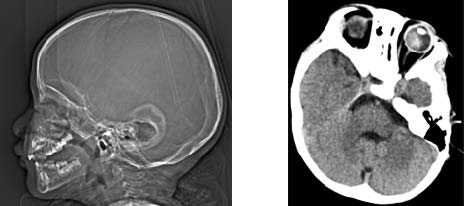
\includegraphics{./images/Image00417.jpg}
 \captionsetup{justification=centering}
 \caption{左侧视网膜母细胞瘤}
 \label{fig7-2-1}
  \end{figure} 

\textbf{【病史摘要】}  男性,3岁。左眼视物模糊。体格检查:左眼白瞳症。

\textbf{【X线表现】}
 左侧眼球中央可见圆形高密度致密灶,呈斑片状,边界清楚,左侧眼眶增大。

\textbf{【X线诊断】}  左侧视网膜母细胞瘤。

\textbf{【评  述】}
 视网膜母细胞瘤是儿童眼内最常见的恶性肿瘤,多发于7岁以下。主要X线表现为球内钙化,钙化率达80%,平片显示率仅为10%,早期呈细沙粒状,以后进展为斑块状,钙化常位于球内肿瘤组织中,但也可向球外或眶外蔓延;视神经孔扩大,双侧视神经孔差异超过10%或1mm提示异常,视神经孔呈圆形,扩大后边缘骨质变薄,是肿瘤向颅内浸润生长的重要标志;其他还有眼眶密度增高,眼眶窝均匀性增大等表现。

\subsection{视神经胶质瘤}

\begin{figure}[!htbp]
 \centering
 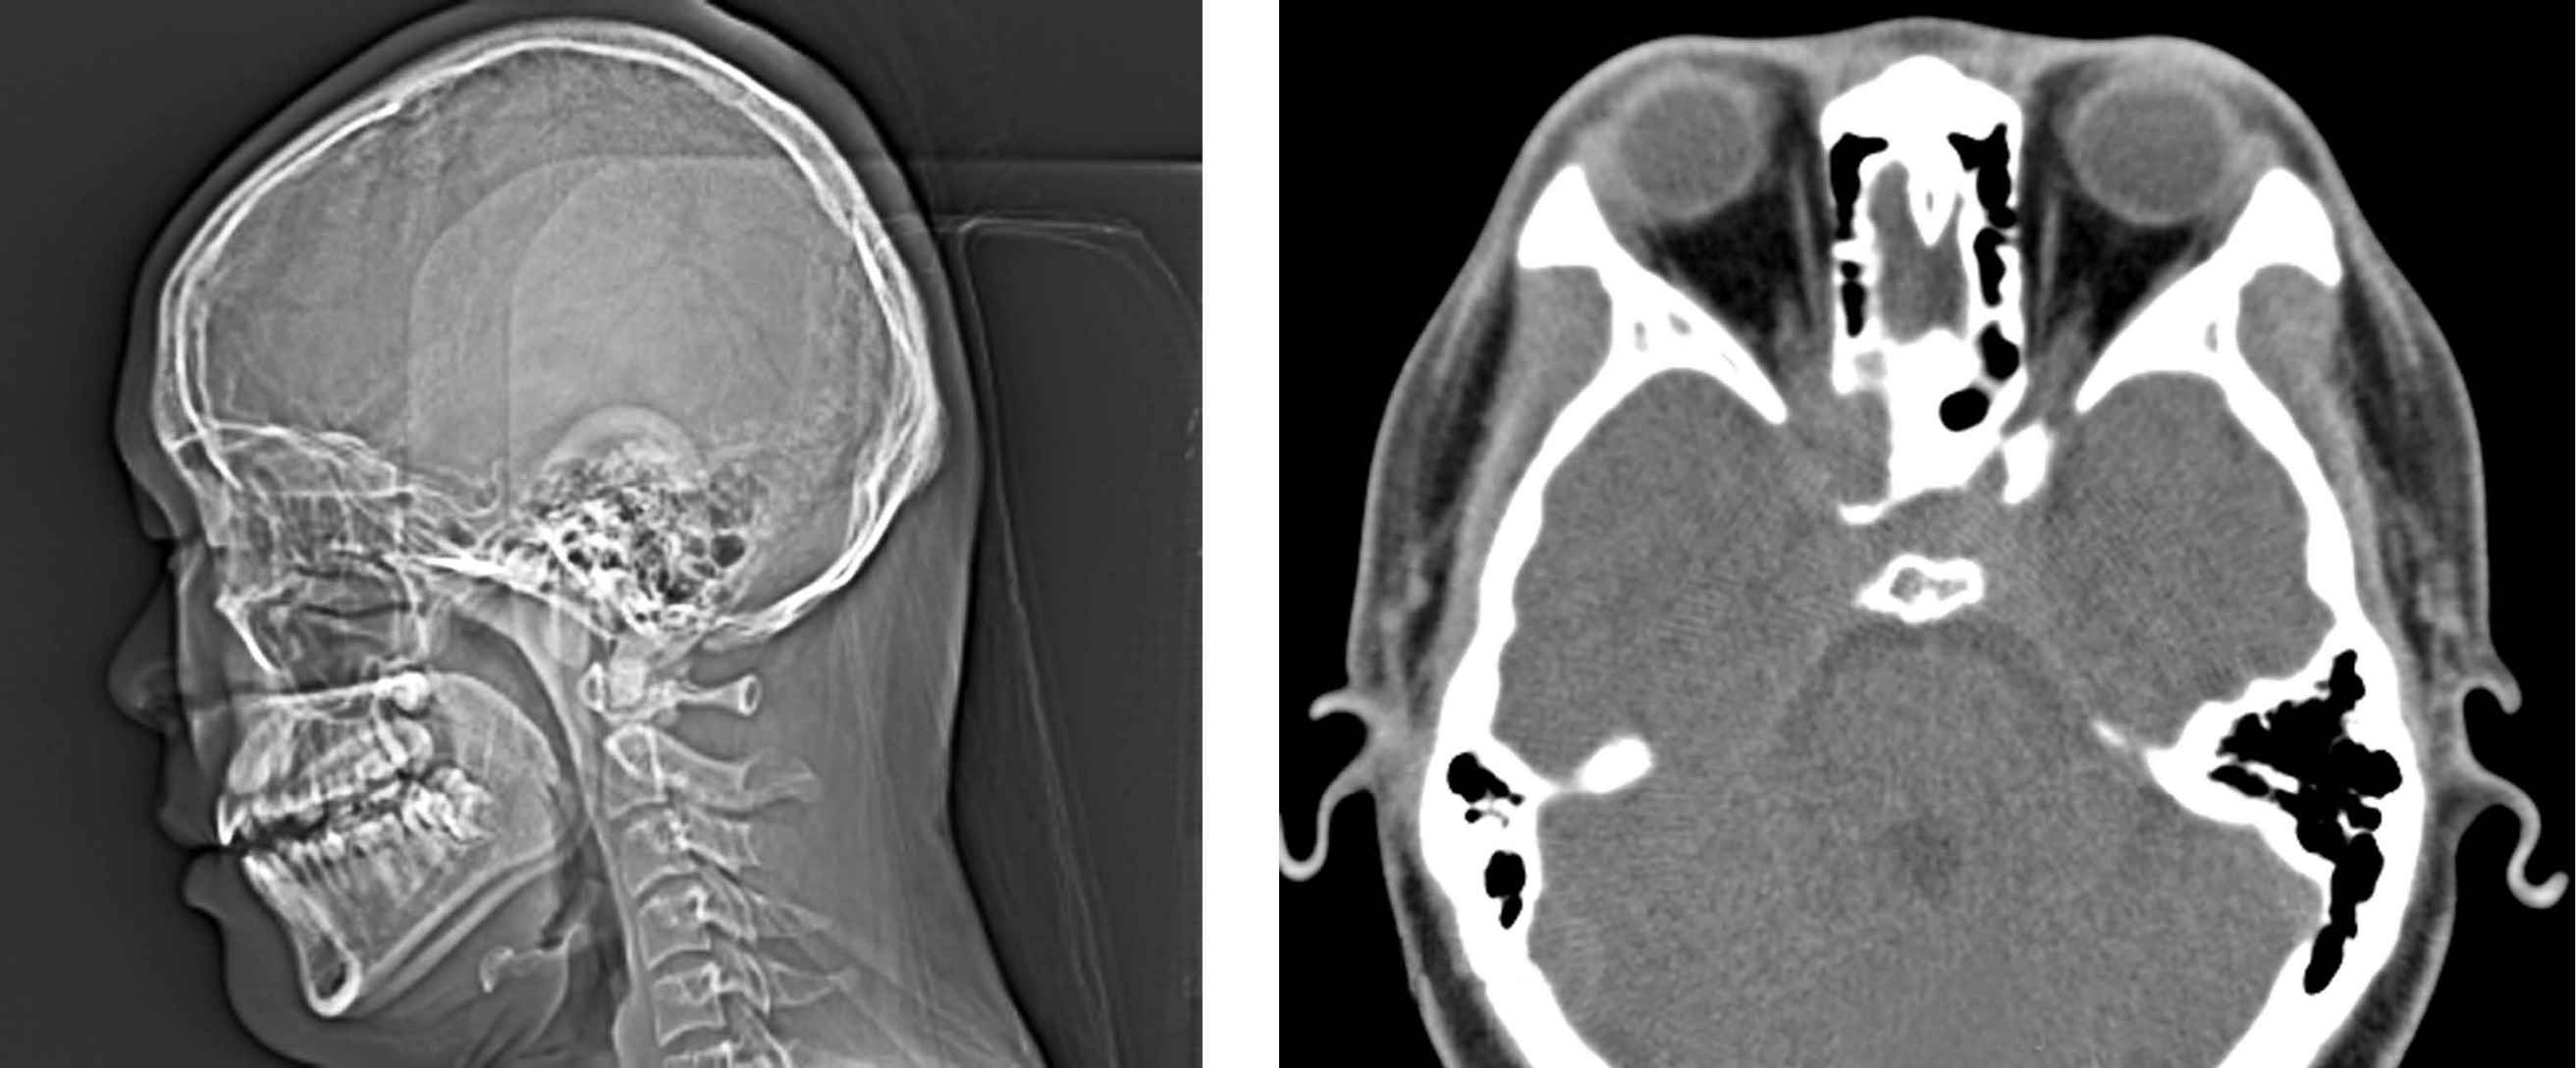
\includegraphics{./images/Image00418.jpg}
 \captionsetup{justification=centering}
 \caption{右侧视神经胶质瘤累及视神经管}
 \label{fig7-2-2}
  \end{figure} 

\textbf{【病史摘要】}  男性,16岁。右眼视力下降5天,视野模糊。

\textbf{【X线表现】}
 双侧眼球等大,球壁光整,右侧视神经孔扩大,较左侧增大2倍左右,骨质边缘光滑清晰而无骨质硬化。

\textbf{【X线诊断】}  右侧视神经胶质瘤累及视神经管内段。

\textbf{【评  述】}
 视神经胶质瘤是原发于视交叉或视神经的良性或低度恶性肿瘤。多发于儿童,临床表现为单眼或双眼视力减退,视野模糊,眼球突出,且视力减退多发生于眼球突出之前。视神经胶质瘤累及视神经管内段时,X线表现为视神经孔扩大,可达对侧孔径的2~4倍,而边缘骨质正常,无骨质硬化。眼眶轻度或中度扩大,少数可引起视交叉沟加深、扩大和蝶鞍变形。进展期可向颅内侵犯,视交叉沟向后凹陷,鞍结节变平,蝶鞍呈W形表现。需要与视神经胶质瘤鉴别的病变主要包括:视神经鞘脑膜瘤、视神经炎、视神经转移瘤和视神经蛛网膜下腔扩大等,仅凭普通X线检查,诊断此病较难,应结合CT及MRI检查。

\subsection{眼眶脑膜瘤}

\begin{figure}[!htbp]
 \centering
 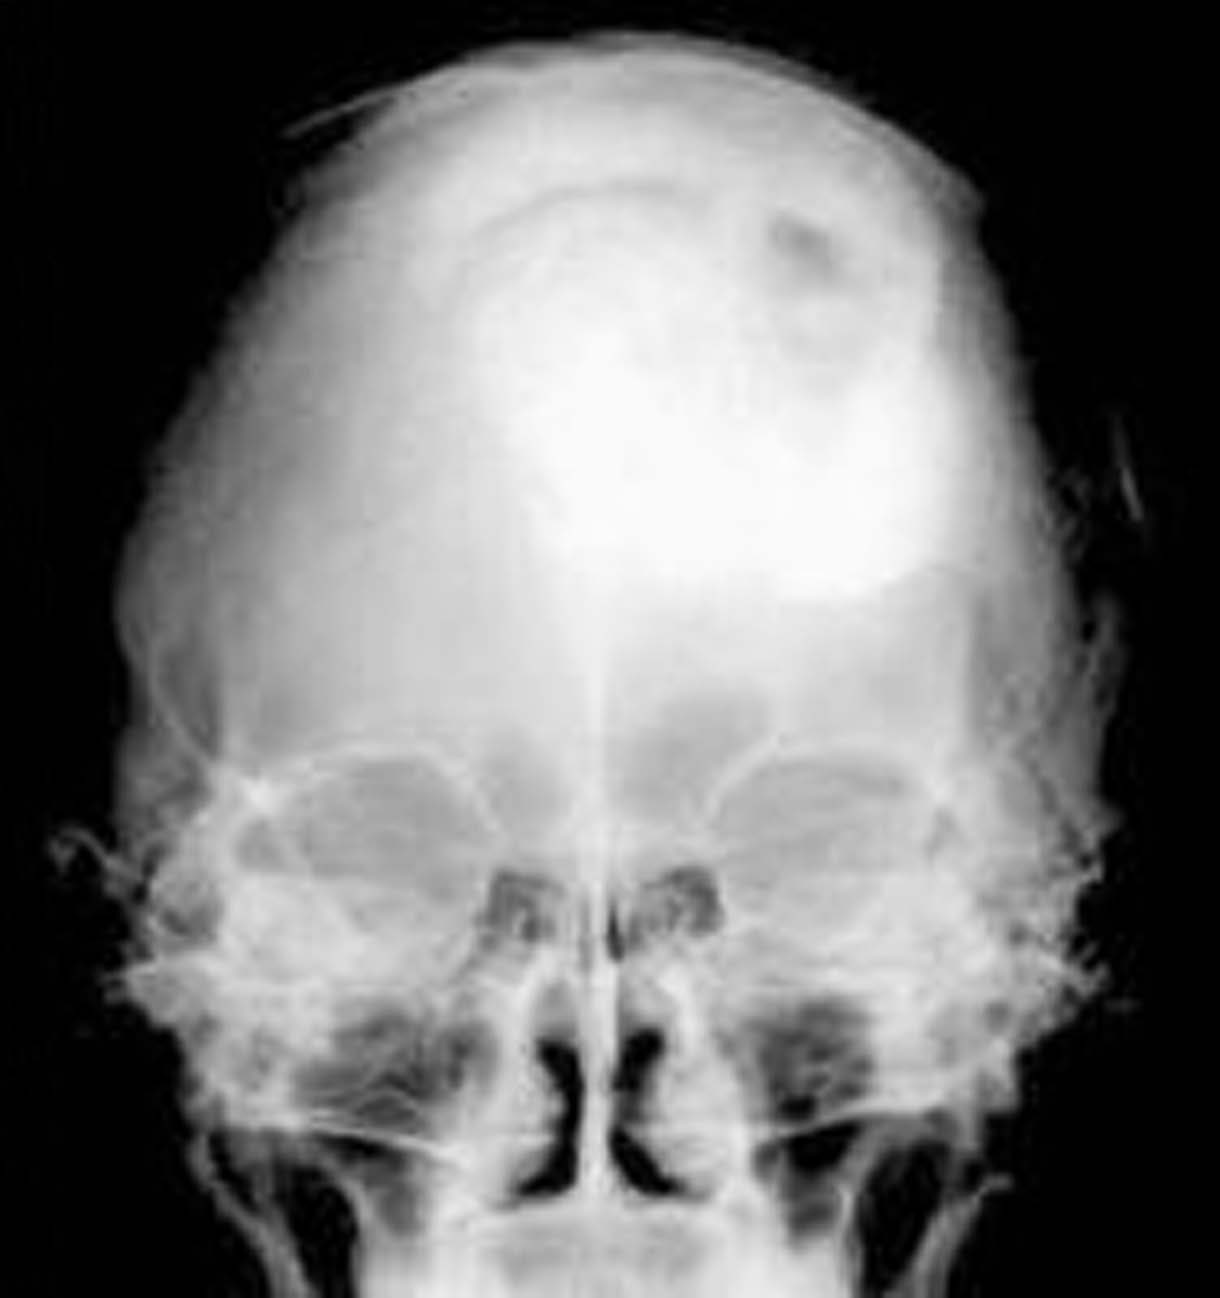
\includegraphics{./images/Image00419.jpg}
 \captionsetup{justification=centering}
 \caption{右侧眼眶脑膜瘤}
 \label{fig7-2-3}
  \end{figure} 

\textbf{【病史摘要】}
 女性,45岁。右眼眼球外凸1年余,伴视力模糊、视力减退。

\textbf{【X线表现】}
 右侧眼眶稍扩大,底部可见扁圆形稍高密度软组织影,附着在眶壁上,边界较清楚。

\textbf{【X线诊断】}  右侧眼眶脑膜瘤。

\textbf{【评  述】}
 眶内脑膜瘤包括原发性和继发性。原发性非常少见,包括视神经管脑膜瘤、神经鞘脑膜瘤及眶内脑膜瘤,多见于中年女性。临床首先表现为视力减退,然后进行性眼球突出。X线表现:①视神经管脑膜瘤,表现为视神经孔周、眶尖或前床突骨膜增生,孔腔轮廓不规则缩小;②周围型脑膜瘤局部眶骨骨膜增生,眼眶增大伴眶内肿块钙化灶,偶见眶上裂扩大。继发性的常来源于蝶骨翼或颅前窝底,临床症状与原发性类似,X线表现为局部骨质增生,呈扁平状或骨瘤状,极少数引起骨质破坏。

\subsection{眼眶神经纤维瘤}

\begin{figure}[!htbp]
 \centering
 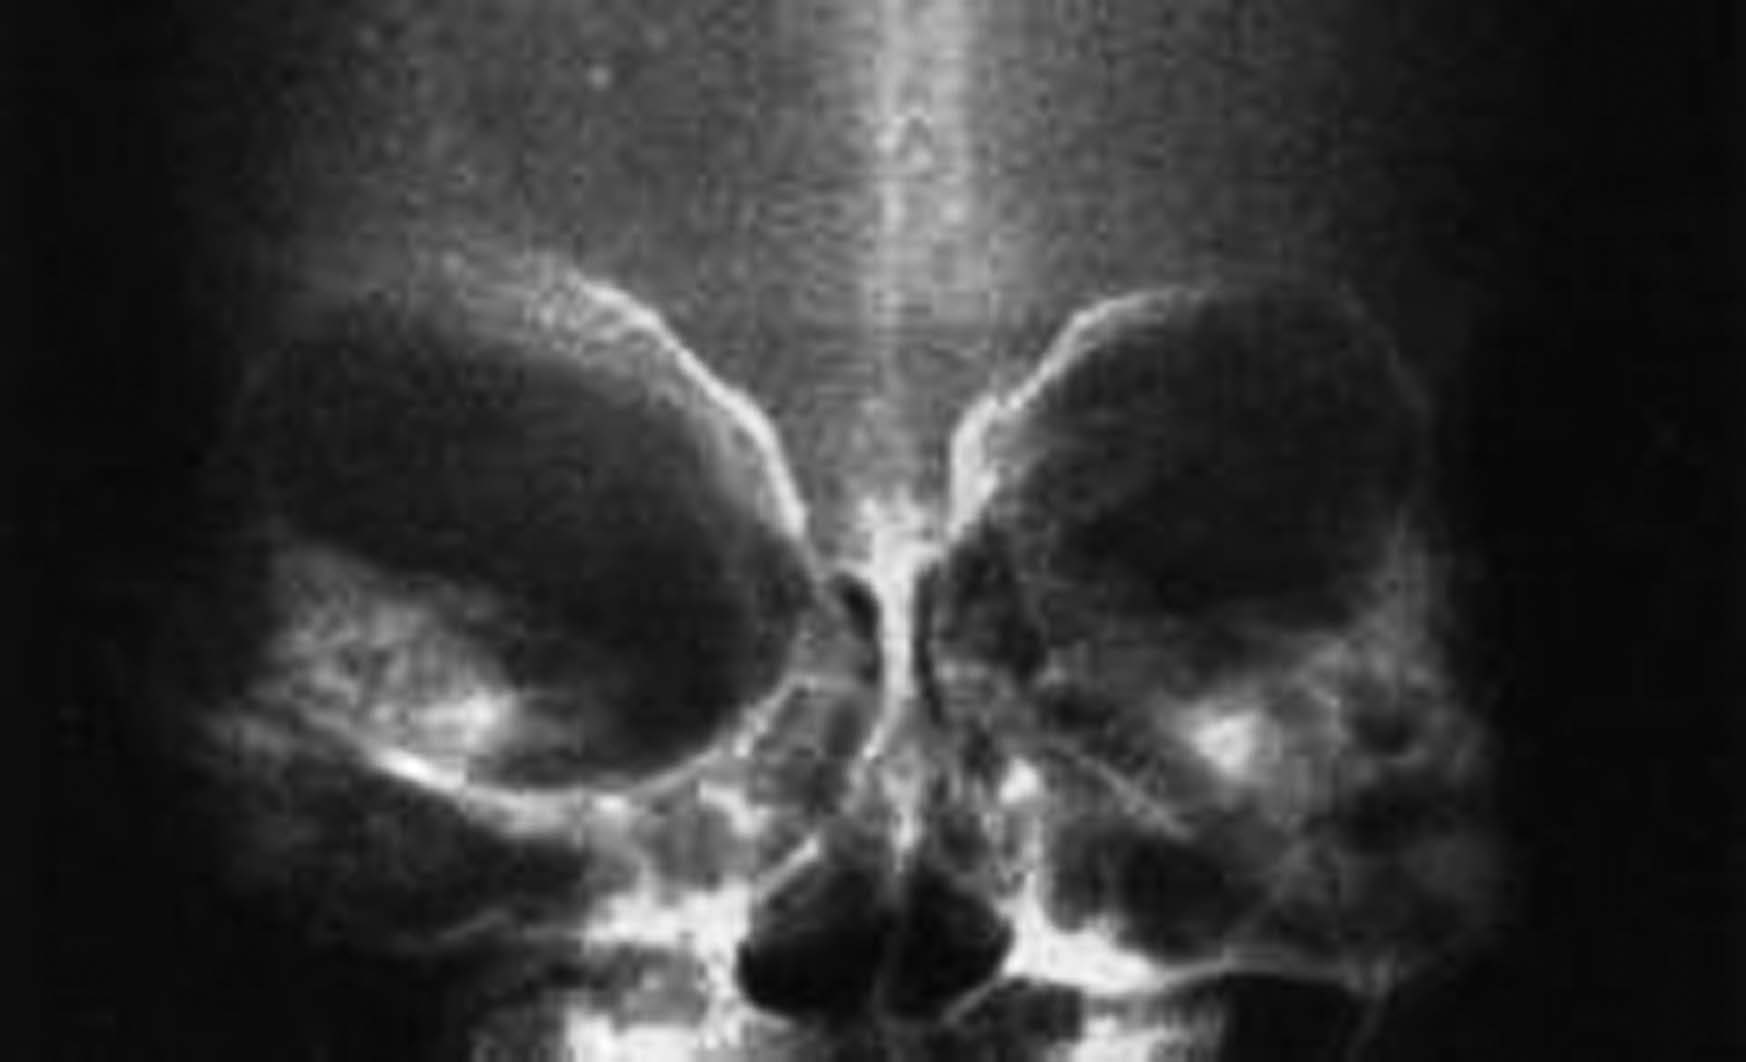
\includegraphics{./images/Image00420.jpg}
 \captionsetup{justification=centering}
 \caption{眼眶神经纤维瘤}
 \label{fig7-2-4}
  \end{figure} 

\textbf{【病史摘要】}
 男性,25岁。右侧眼球向前方外凸,视力较前明显下降。

\textbf{【X线表现】}
 右侧眼眶增大,眼眶底部可见不规则高密度影,边界欠清楚,附着在眼眶壁下缘。

\textbf{【X线诊断】}  右侧眼眶神经纤维瘤。

\textbf{【评  述】}
 眼眶神经纤维瘤属于神经外胚层肿瘤,瘤内多种神经组织成分增生,以神经鞘膜细胞核显微组织为主。临床上分为孤立性和丛状神经纤维瘤。多发于青中年。神经纤维瘤病常见眼眶和颅底骨发育障碍,以蝶骨为中心,主要表现为蝶骨大翼骨缺损,蝶骨小翼骨很小,眶上裂扩大或伴眼眶普遍性扩大,颞骨缺损。X线表现为稍高密度软组织肿块影,有时伴随眼眶变大,以眶顶区为著。X线表现特异性不大。诊断应结合CT、MRI及临床表现综合分析。

\subsection{眼眶异物}

\begin{figure}[!htbp]
 \centering
 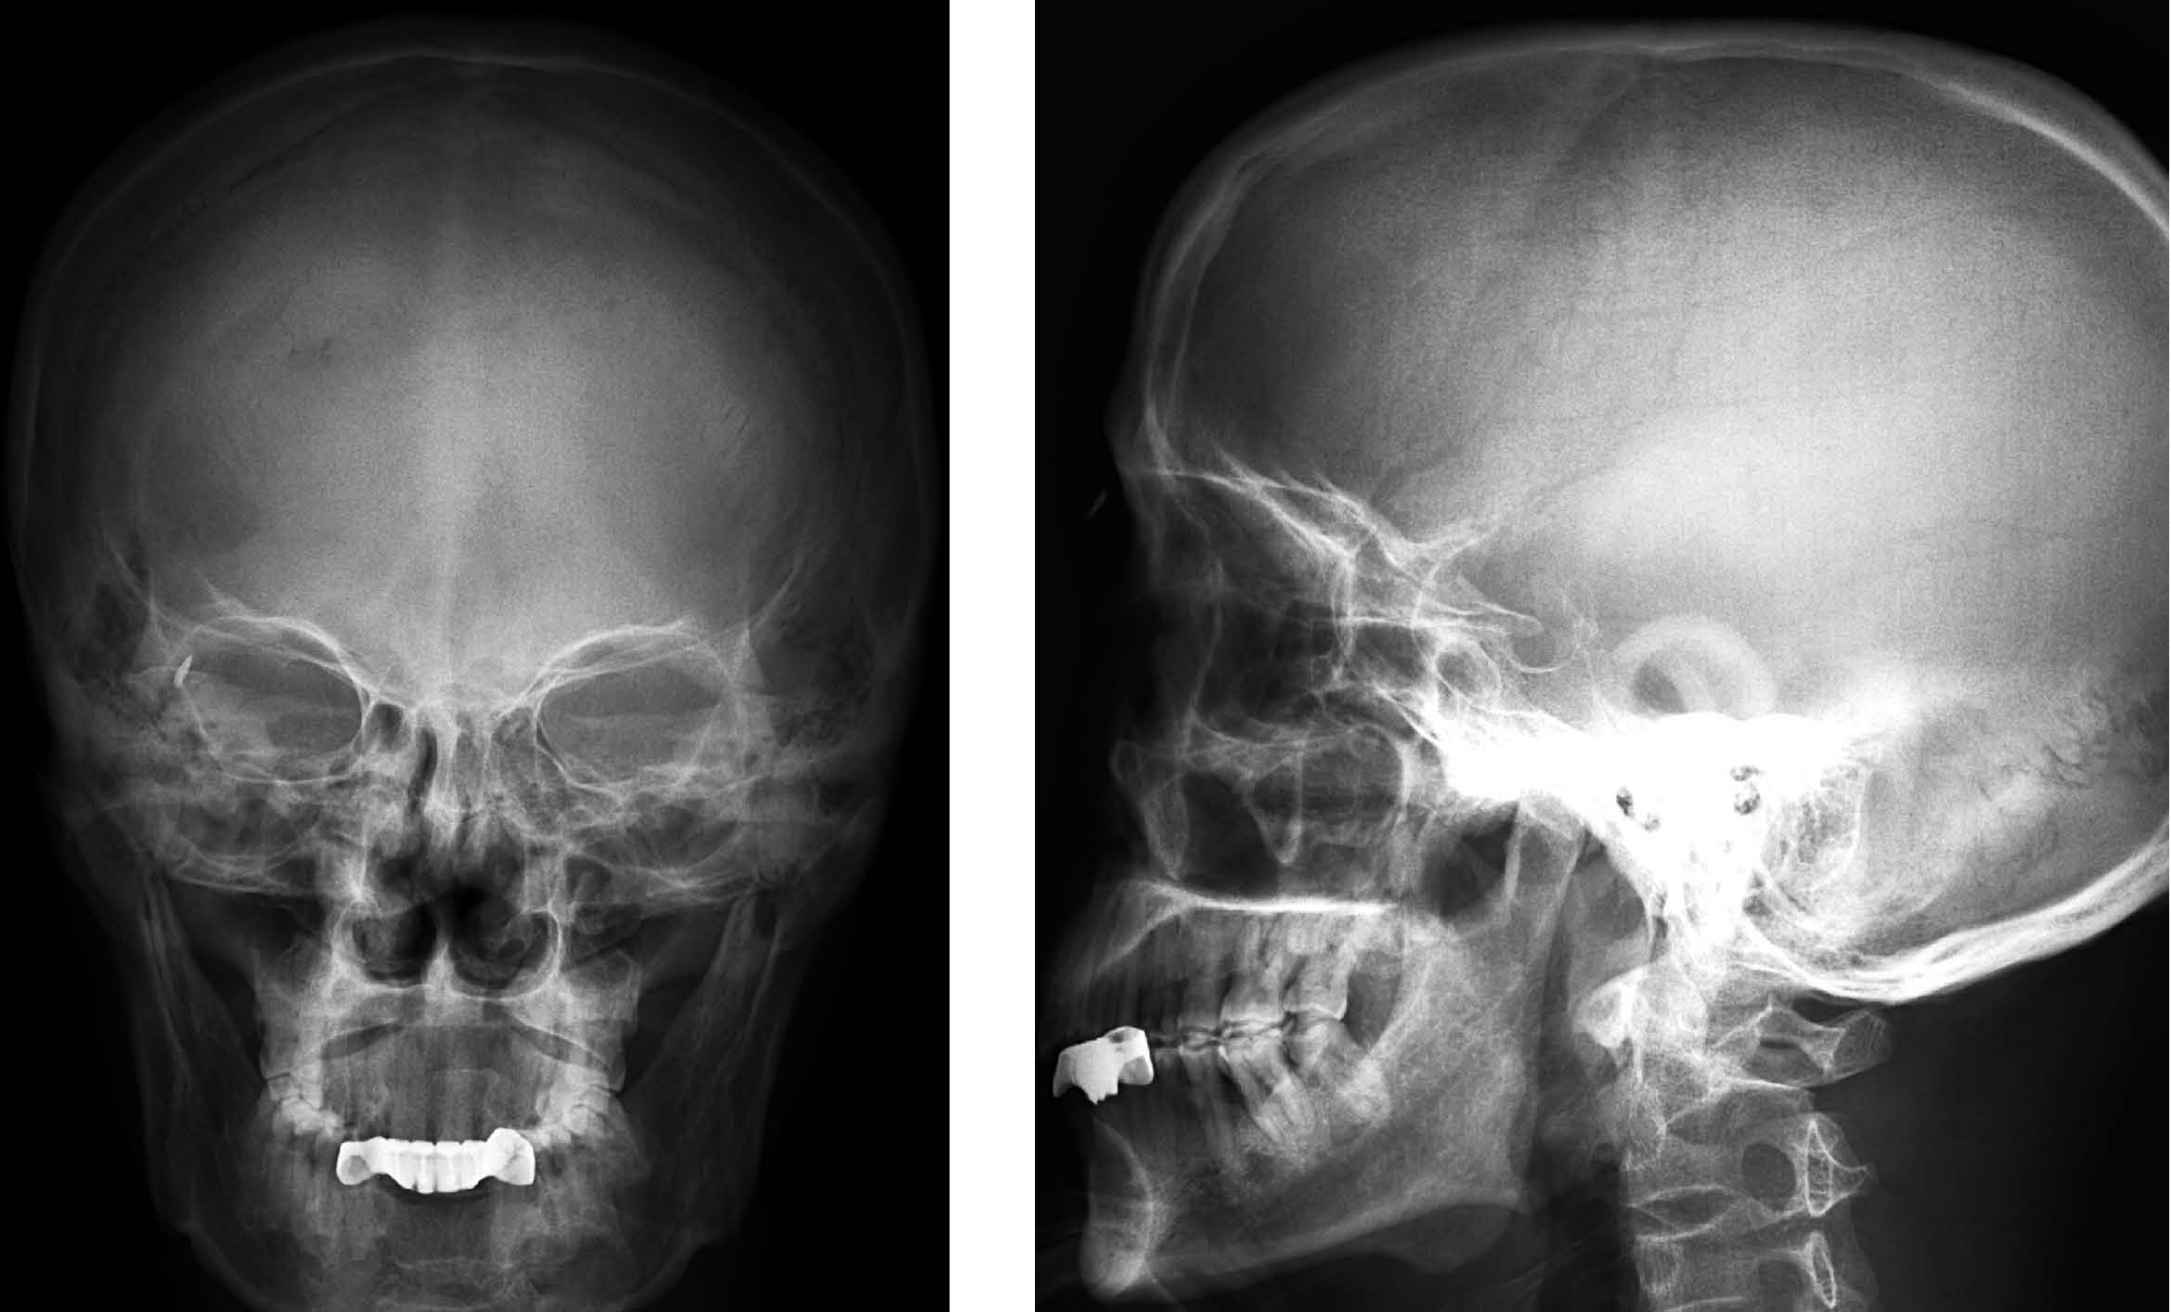
\includegraphics{./images/Image00421.jpg}
 \captionsetup{justification=centering}
 \caption{眼眶异物}
 \label{fig7-2-5}
  \end{figure} 

\textbf{【病史摘要】}
 男性,54岁。刨木屑致右眼眶损伤,出现异物感约1周。

\textbf{【X线表现】}
 右侧眼眶壁外侧缘可见条状高密度影,侧位片示病灶位于眼窝内。

\textbf{【X线诊断】}  右侧眼眶异物。

\textbf{【评  述】}
 X线平片可以确定异物的存在,若不能确定眼球内外异物时做X线定位检查。包括确定异物在眼球的位置,鉴别异物在球内还是球外,测定异物对应于巩膜表面的位置、异物在球内是否移动等。其中直接定位法较简单,定位误差在2mm之内,能满足一般临床需求。

\subsection{泪腺肿瘤}

\begin{figure}[!htbp]
 \centering
 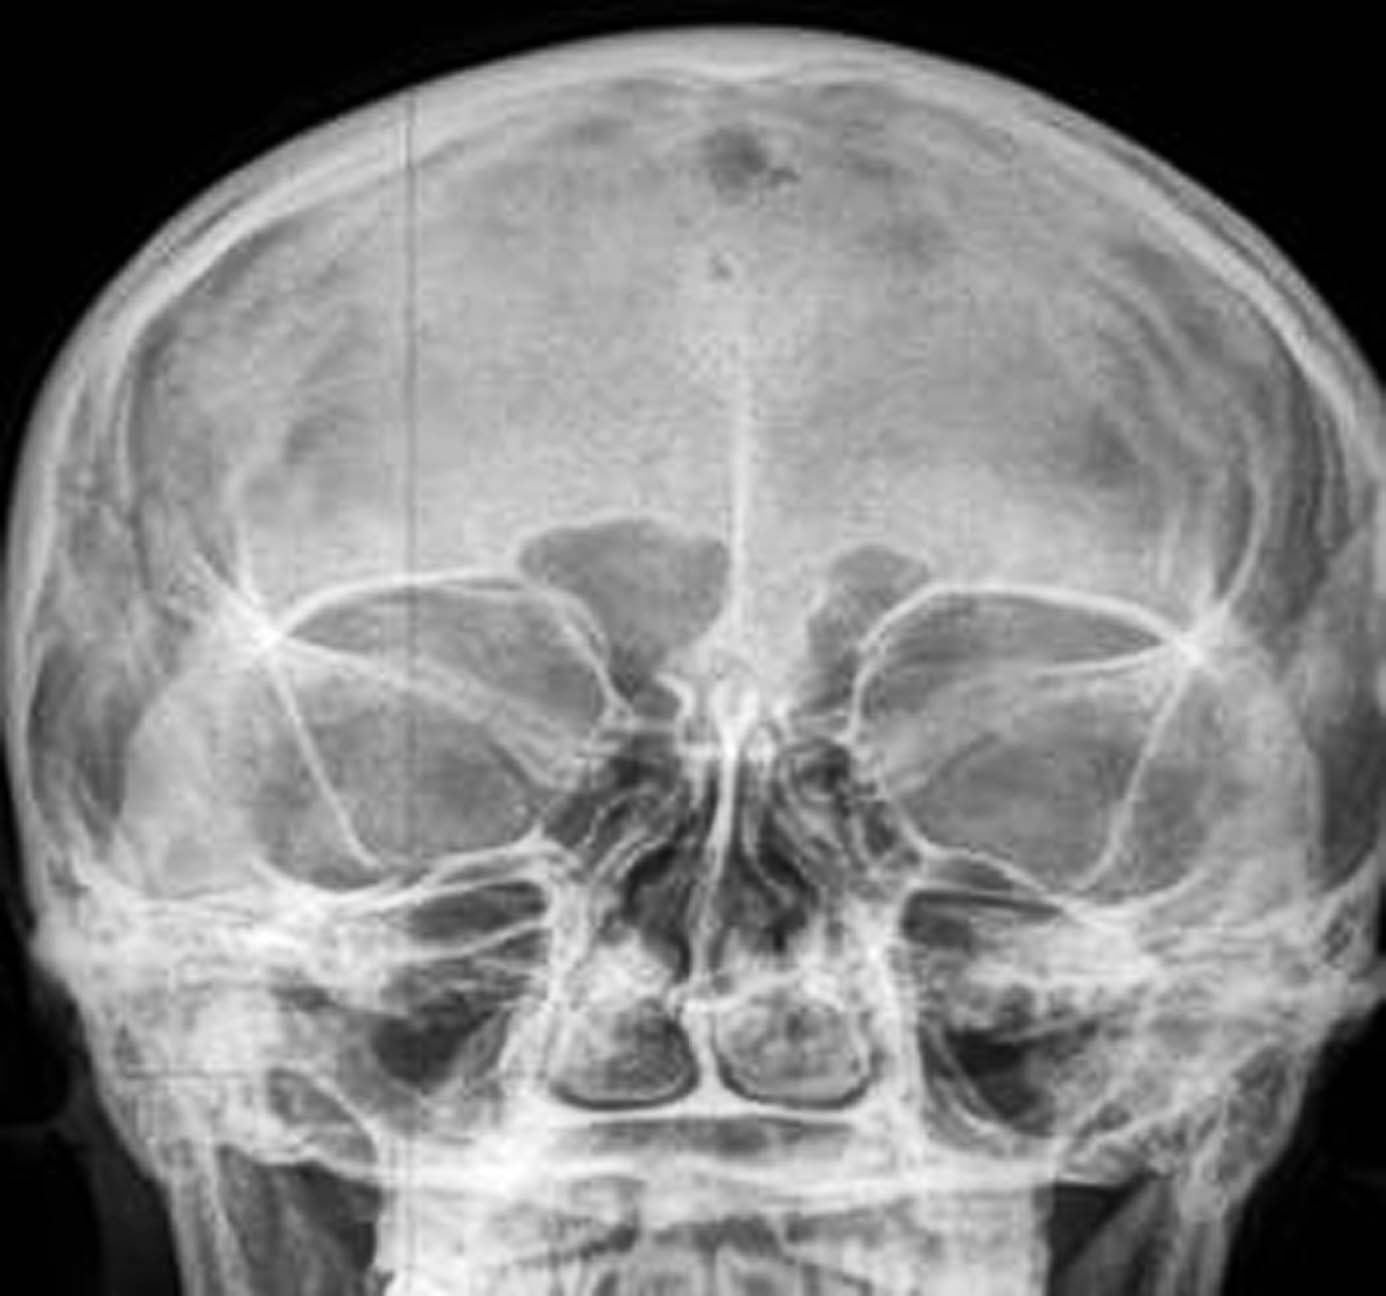
\includegraphics{./images/Image00422.jpg}
 \captionsetup{justification=centering}
 \caption{左侧泪腺混合瘤}
 \label{fig7-2-6}
  \end{figure} 

\textbf{【病史摘要】}
 女性,38岁。左侧眼球轻度突出,并向内下移位,视力下降。

\textbf{【X线表现】}
 左侧眼眶稍增大,眶内外上方密度增高,局部眶骨皮质欠光整。泪腺窝增大。

\textbf{【X线诊断】}  左侧泪腺混合瘤。

\textbf{【评  述】}
 泪腺肿瘤来源于泪腺或副泪腺,大多为良性的混合瘤,少数为腺癌。好发于中年人,良性生长缓慢,临床表现为睑外侧隆起或伴突眼向内下方。X线最常见的表现为眼眶外上方的泪腺窝变形和扩大;骨质破坏,混合瘤主要表现为局部或边缘骨质吸收,癌则表现为泪腺边缘模糊或骨质吸收,破坏多局限于泪腺窝,进展期可侵犯额骨、眼锥、视神经孔和颅底;骨膜硬化,泪腺窝及眶外上方骨质硬化,为骨膜受累表现;眼眶普遍扩大,常发生于病程长的或较大的肿瘤。

\subsection{眶内海绵状血管瘤}

\begin{figure}[!htbp]
 \centering
 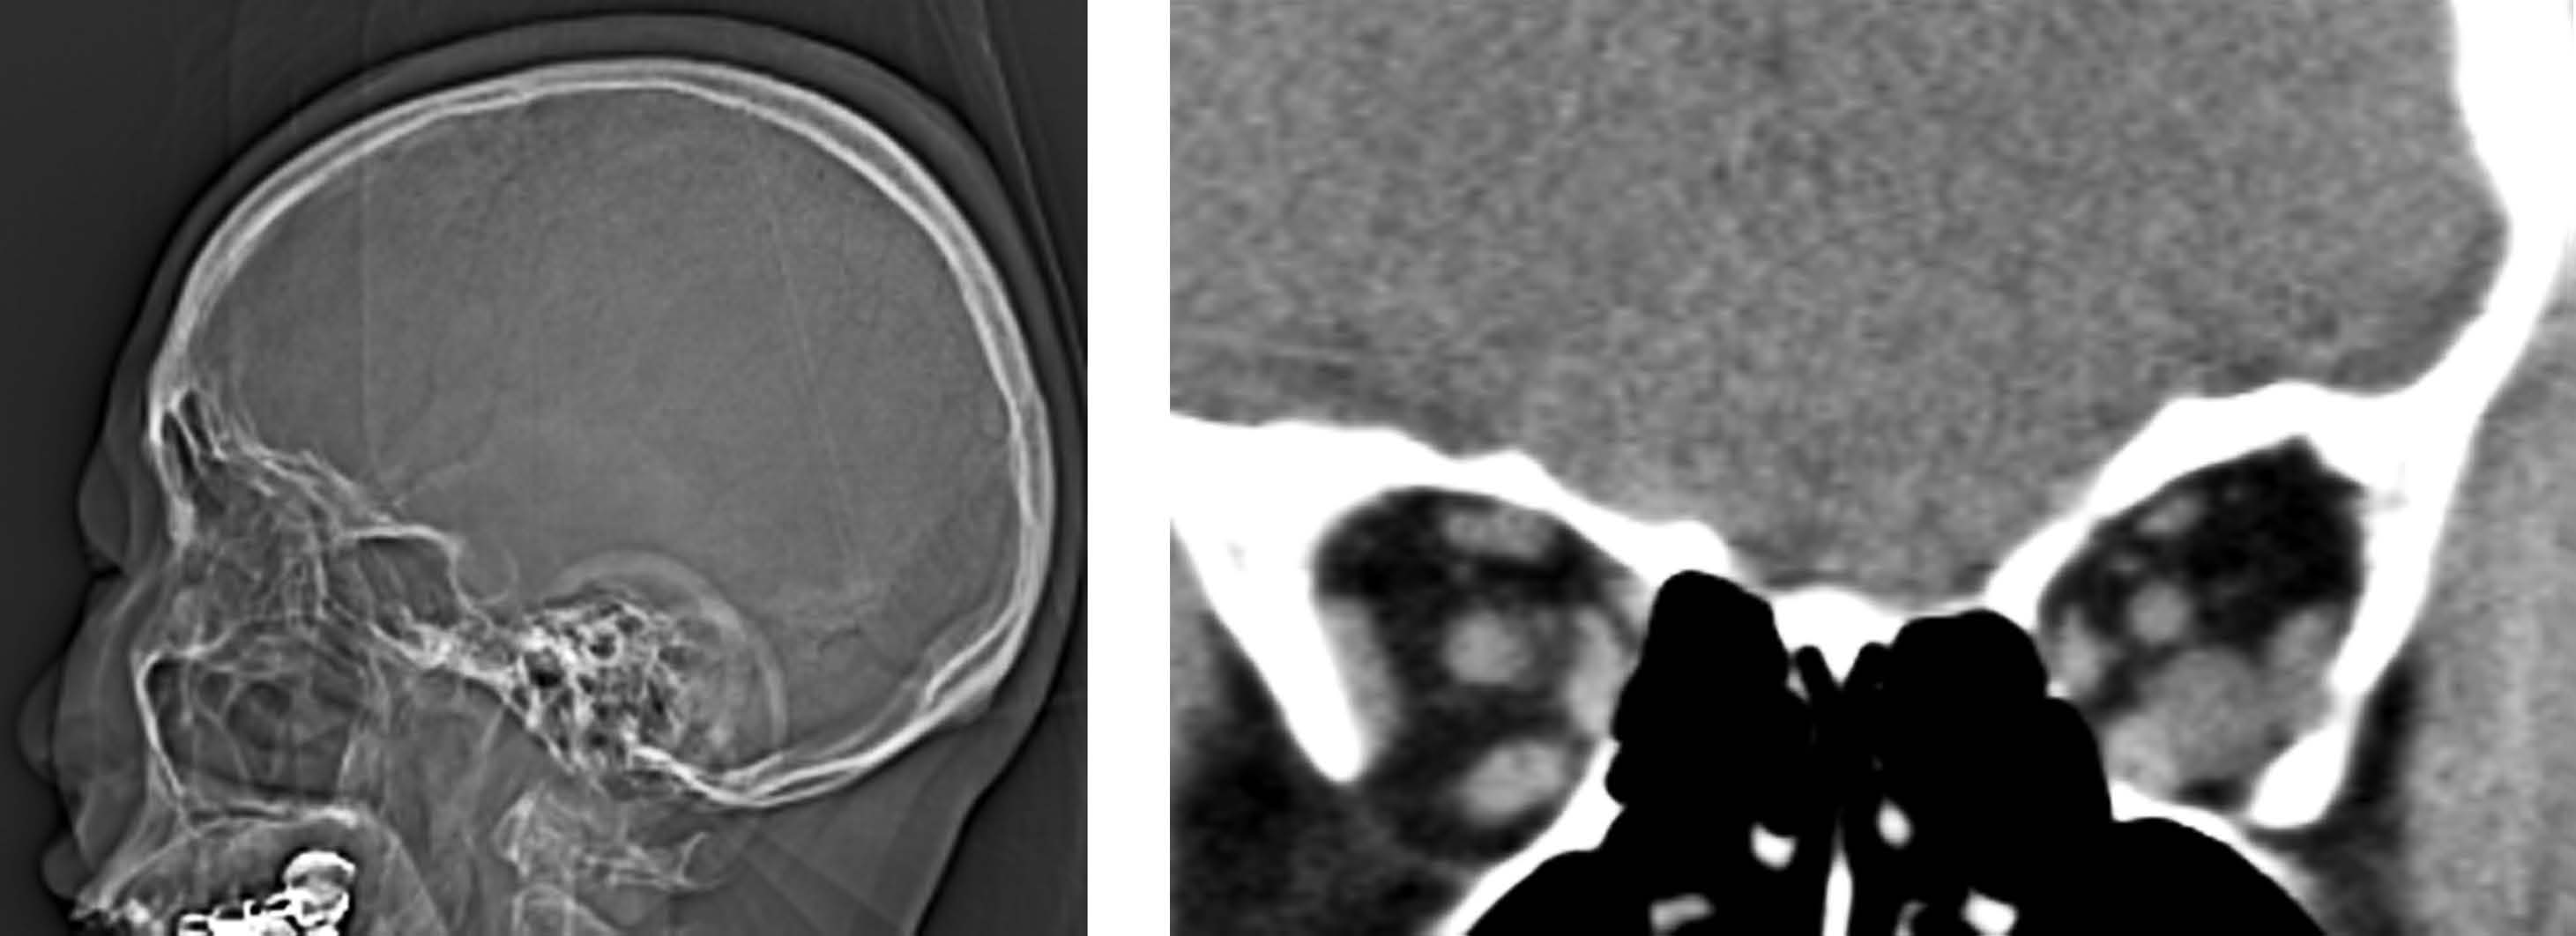
\includegraphics{./images/Image00423.jpg}
 \captionsetup{justification=centering}
 \caption{左侧眶内海绵状血管瘤}
 \label{fig7-2-7}
  \end{figure} 

\textbf{【病史摘要】}
 女性,54岁。左眼先天性上睑下垂,视力未见明显改变。

\textbf{【X线表现】}
 左侧眼眶侧位片示左侧眼眶稍增大,其下方似见类圆形稍高密度影,边缘尚光整,周围骨质未见明显破坏、硬化。CT冠状位片示左侧下直肌上方椭圆形软组织密度影,边缘光整,有一定占位现象。

\textbf{【X线诊断】}  左侧眶内海绵状血管瘤。

\textbf{【评  述】}
 海绵状血管瘤是成人眶内最常见的良性肿瘤,常于中青年时期发病,女性稍多。肿瘤多位于眼眶肌锥内,绝大多数为单发,极少数为多发,生长缓慢,视力一般不受影响。常见体征为无痛性、慢性进行性眼球突出。X线表现为眼眶扩大,特征性的表现是眼眶内可见静脉石和斑片状钙化。普通X线片对于眶内海绵状血管瘤的诊断较难,应结合CT及MRI检查。CT主要表现为肌锥内圆形或椭圆形病灶,边界清楚。大部分肿瘤与眼外肌等密度,且密度均匀,少数可见小圆形高密度钙化,为静脉石,增强后呈中重度强化。MRI检查海绵状血管瘤T\textsubscript{1}
WI呈低信号或等信号,T\textsubscript{2}
WI呈高信号,信号均匀。动态增强可表现为渐进性强化,最终整个肿瘤明显均匀强化,此表现为诊断海绵状血管瘤的特异征象。

\section{耳病变}

\subsection{急性化脓性中耳炎}

\begin{figure}[!htbp]
 \centering
 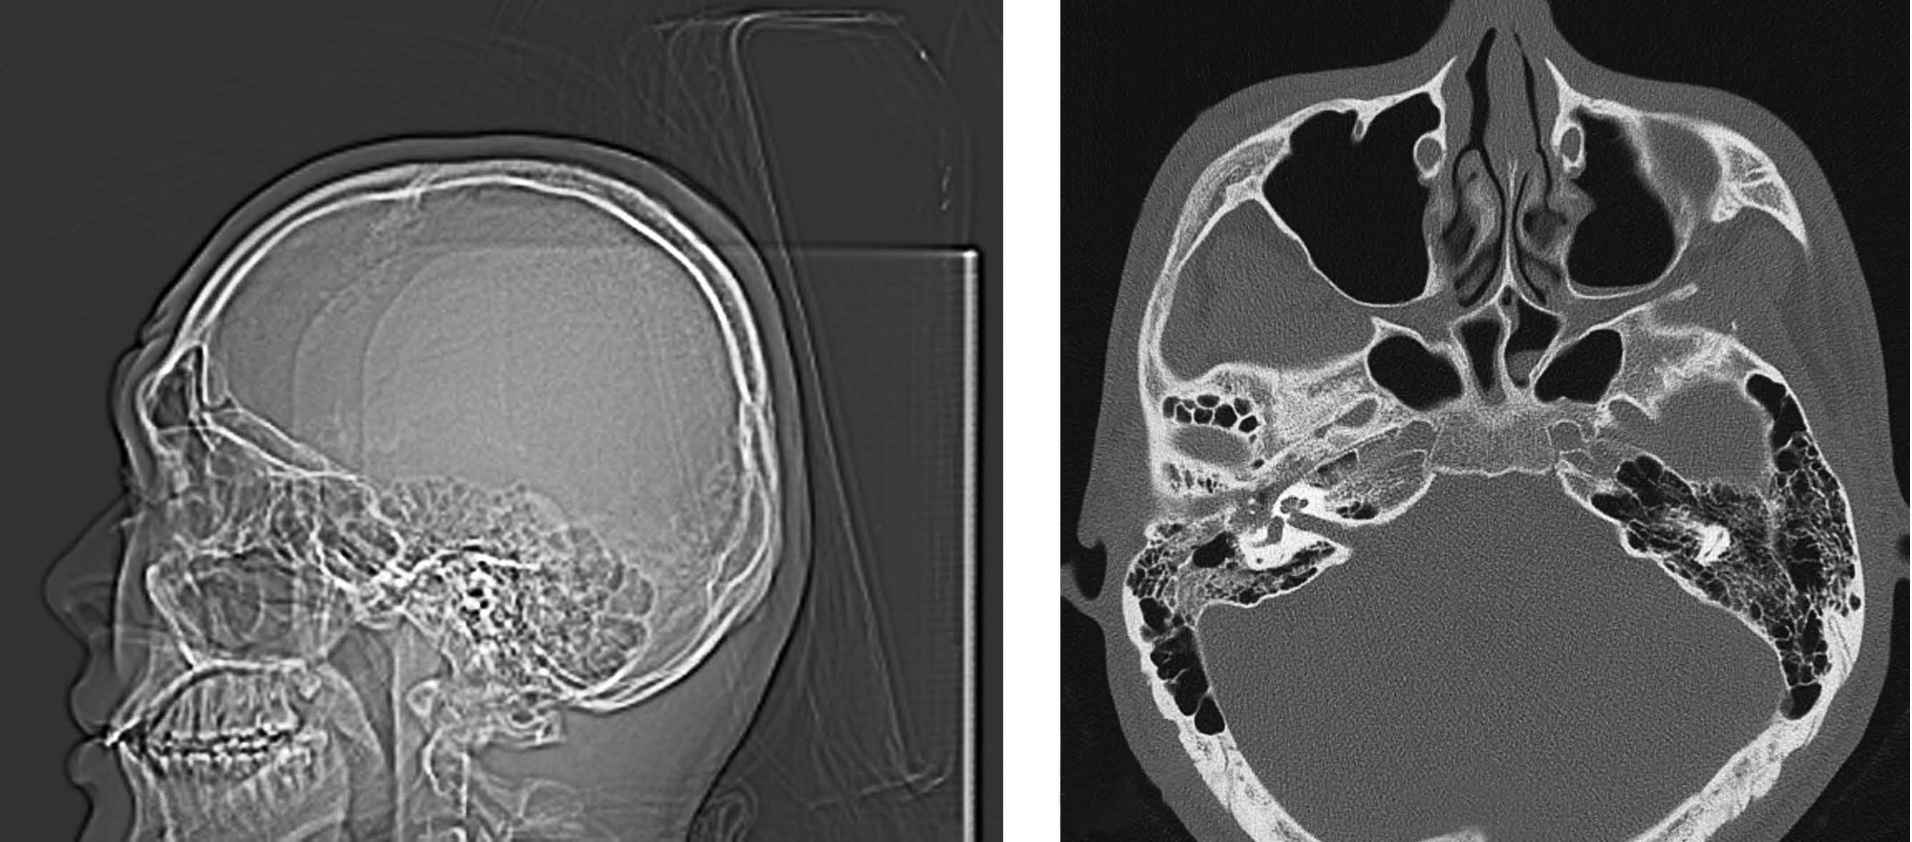
\includegraphics{./images/Image00424.jpg}
 \captionsetup{justification=centering}
 \caption{急性化脓性中耳炎}
 \label{fig7-3-1}
  \end{figure} 

\textbf{【病史摘要】}
 男性,18岁。双耳流脓10天。体格检查:双侧耳道及耳后软组织肿胀明显。

\textbf{【X线表现】}
 右侧乳突气房透光度减低,密度增高,模糊,小房间隔模糊,鼓窦区无明显骨质破坏。CT横断位示中耳腔内见软组织影。

\textbf{【X线诊断】}  急性化脓性中耳炎。

\textbf{【评  述】}
 本病好发于儿童,炎症常局限于鼓室和鼓窦,一般称为中耳鼓窦炎。临床症状为耳内和耳后深部阵痛或持续疼痛,穿孔后疼痛减轻出现耳漏。X线表现为中耳透亮度减低,早期表现为鼓窦周围的小气房,当气房内气体被炎症病变和积液所替代,气房透亮度减低,呈一片增白表现,骨间隔却正常;当有脓腔形成时,局部网状结构中断,形成相对小片状无结构透亮区。

\subsection{慢性化脓性中耳炎}

\begin{figure}[!htbp]
 \centering
 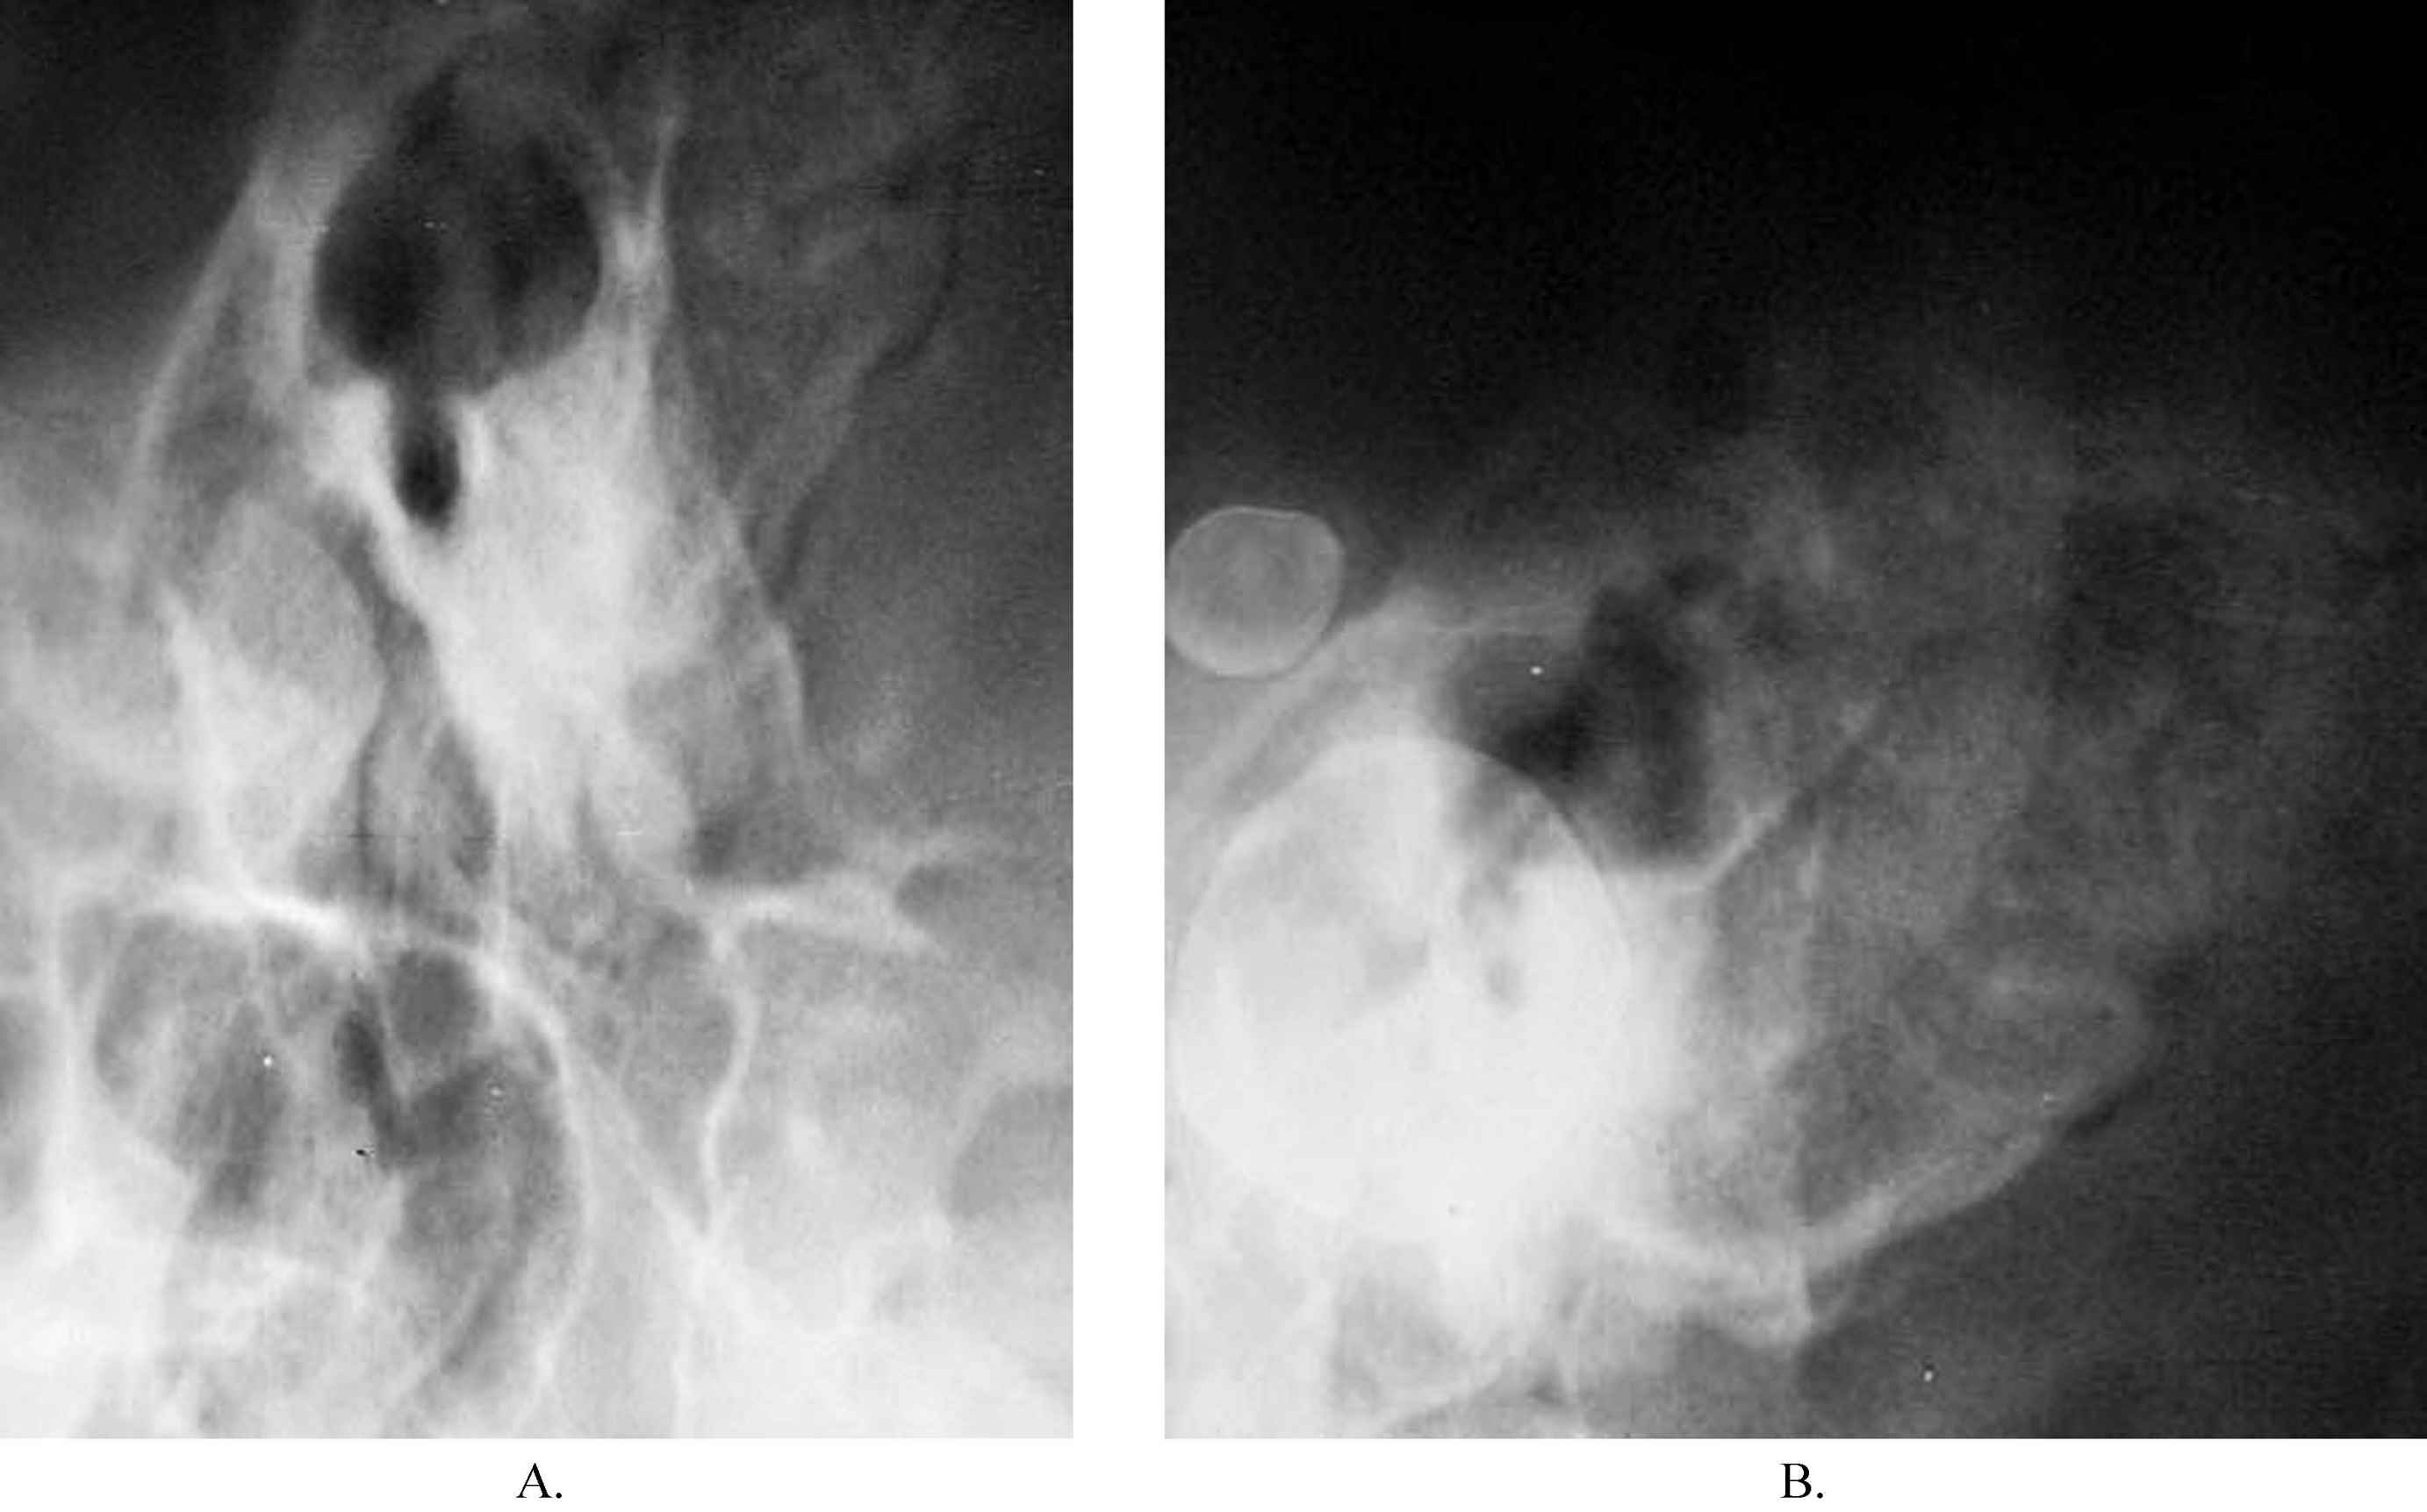
\includegraphics{./images/Image00425.jpg}
 \captionsetup{justification=centering}
 \caption{右耳中耳乳突炎}
 \label{fig7-3-2}
  \end{figure} 

\textbf{【病史摘要】}
 男性,34岁。右耳持续性流脓3个月余,耳痛伴听力下降1个月。

\textbf{【X线表现】}
 图A、图B分别为右乳突梅氏位和许氏位乳突片,鼓窦区可见骨质破坏,部分边缘锐利硬化,鼓窦入口扩大。

\textbf{【X线诊断】}  右耳中耳乳突炎(胆脂瘤型)。

\textbf{【评  述】}
 急性化脓性中耳炎症未能及时治疗或病情较重,治疗后未痊愈,病程超过6~8周则称为慢性中耳炎,临床症状主要为长期间歇性流脓史,伴有不同程度听力障碍。临床分三型:单纯型、肉芽肿型及胆脂瘤型。单纯型表现为鼓窦、中耳腔慢性炎症,透亮度减低,周围骨质硬化,而无上鼓室、入口和鼓窦区的骨破坏,乳突透亮度减低,骨间隔增厚,粗细不均。肉芽肿型多见于板障型乳突,局限于上鼓室,表现为上鼓室扩大,边缘模糊,累及鼓窦入口,则见上鼓室鼓窦入口扩大,侵犯鼓窦后则鼓窦区破坏。胆脂瘤型早期局限于上鼓室,继之进入鼓窦入口、鼓窦及向周围乳突部扩展,形成大的破坏腔,呈透亮区,病灶边缘光滑锐利,可见致密硬化带。

\subsection{中耳癌}

\begin{figure}[!htbp]
 \centering
 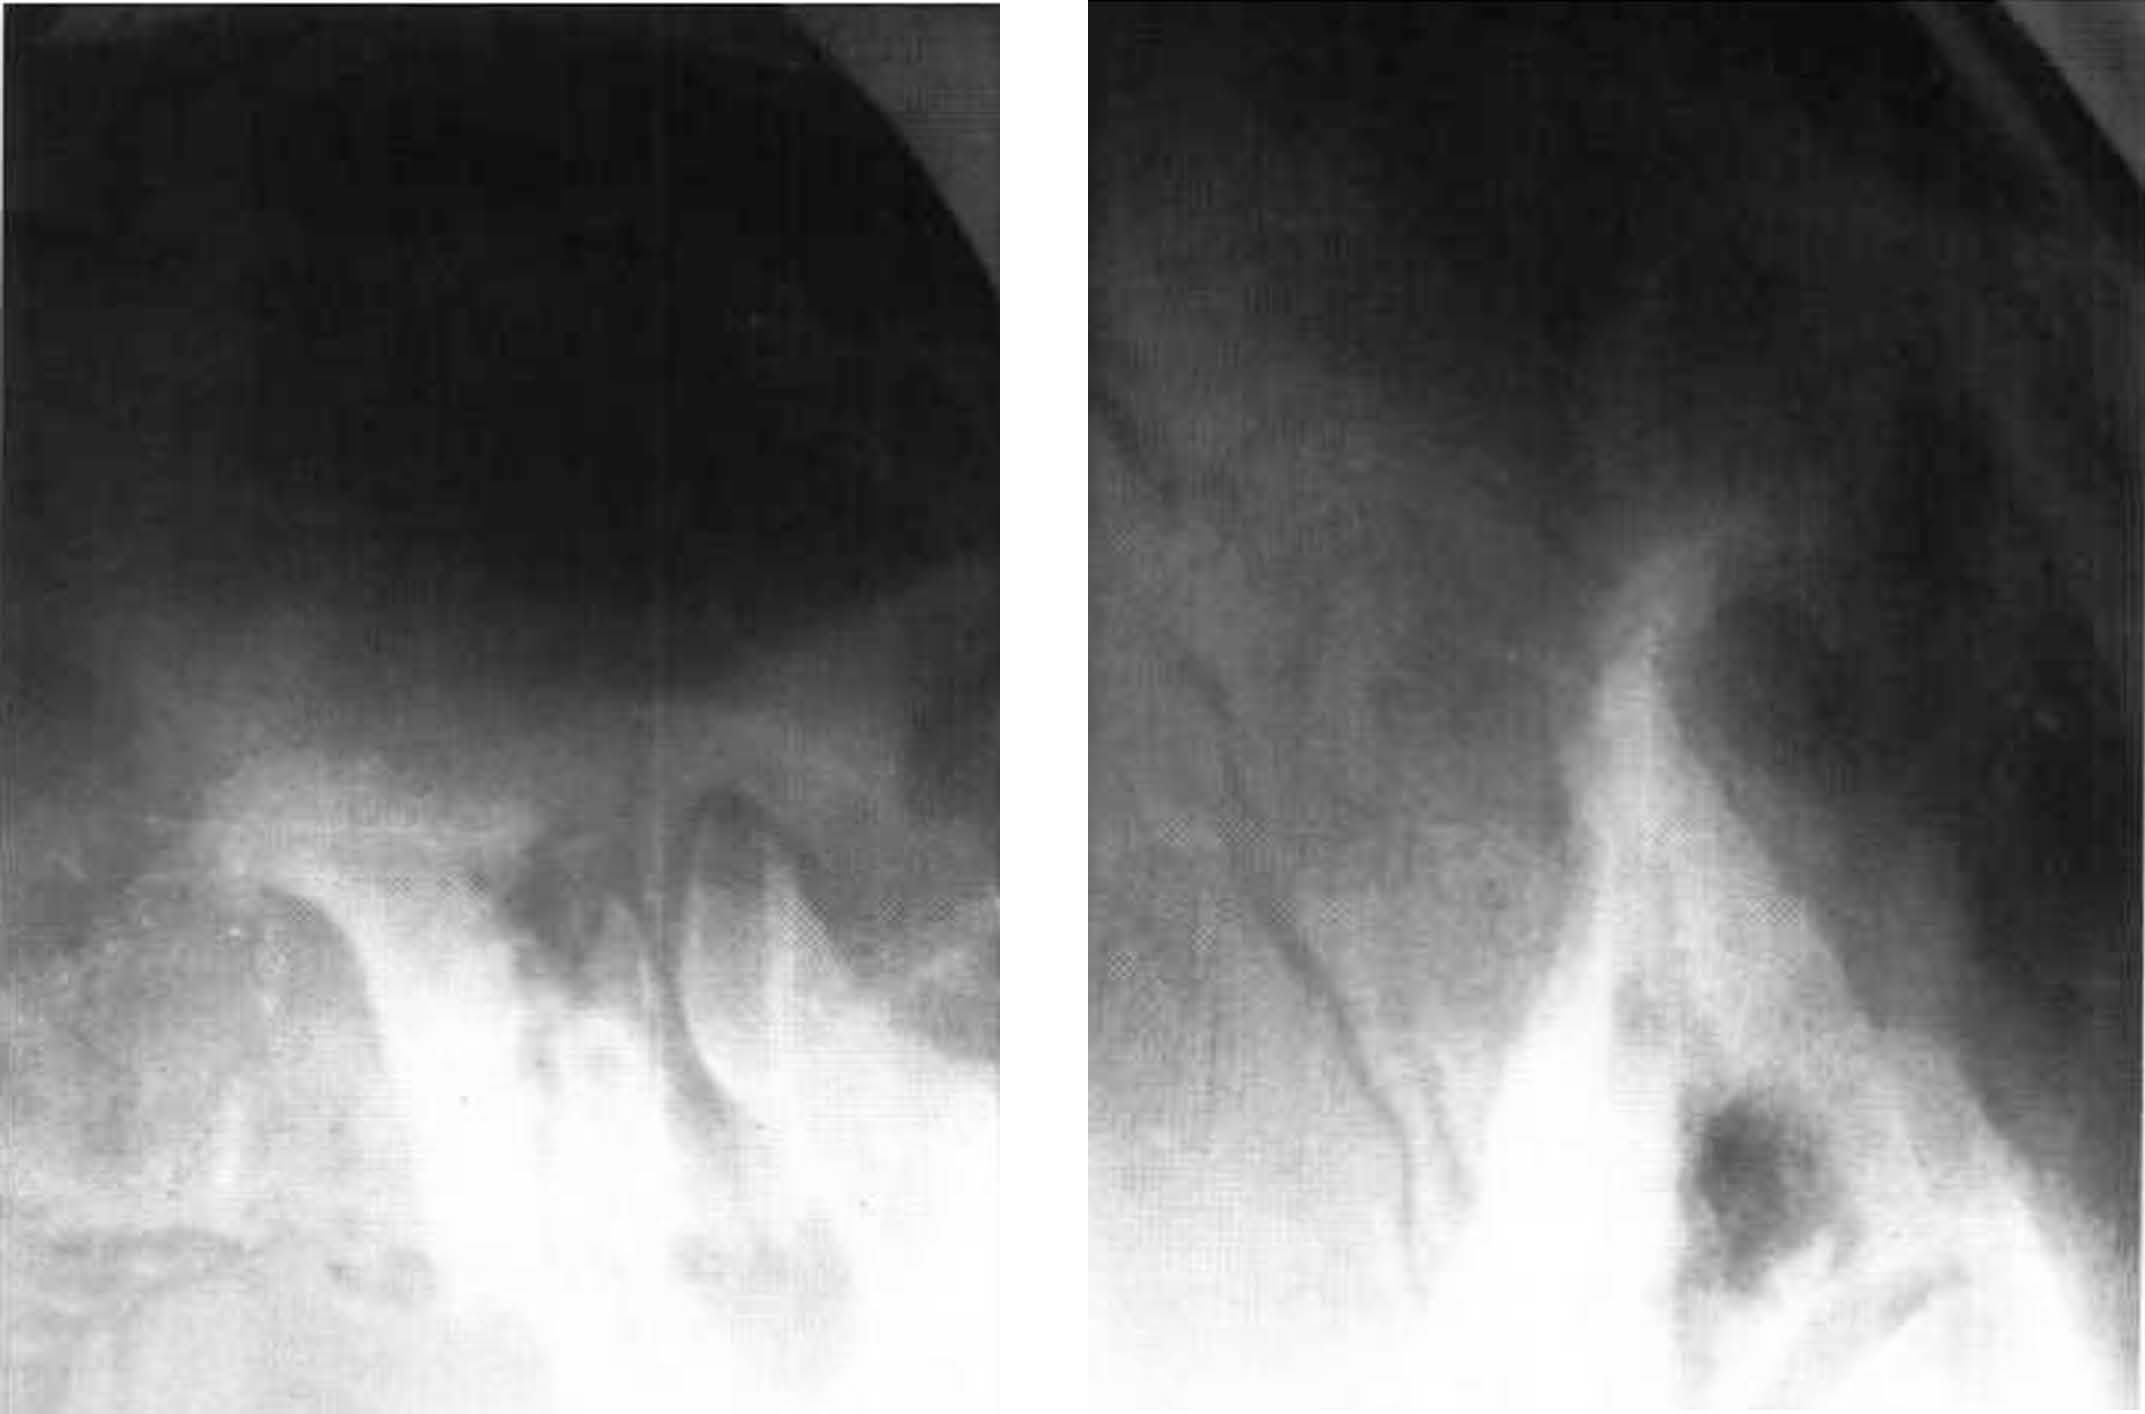
\includegraphics{./images/Image00426.jpg}
 \captionsetup{justification=centering}
 \caption{左侧中耳癌}
 \label{fig7-3-3}
  \end{figure} 

\textbf{【病史摘要】}
 男性,65岁。左耳反复流脓10余年,近来耳痛。体格检查:左侧外耳道见血性分泌物及肉芽组织,左中耳腔积液。

\textbf{【X线表现】}
 左侧乳突密度增高,气房消失。外耳道壁骨质破坏、断裂、外耳孔扩大明显,鼓窦入口及上鼓室骨质吸收,边缘模糊。

\textbf{【X线诊断】}  左侧中耳癌。

\textbf{【评  述】}
 本病多见于中老年人,病理多为鳞癌,少数为基底细胞癌、腺癌。临床表现为耳聋,多见水样或带血或有臭味分泌物,疼痛明显,晚期可有面瘫。中耳癌早期可致听小骨破坏,中耳腔透亮度减低,中耳骨壁稀疏或骨质破坏,咽鼓管骨性段常累及,以颅底片显示较佳。侧斜位片可见上鼓室入口向上扩大,边缘不齐,呈充实状破坏。与慢性中耳炎有时较难鉴别,需结合临床检查。

\section{鼻及鼻旁窦病变}

\subsection{鼻骨骨折}

\begin{figure}[!htbp]
 \centering
 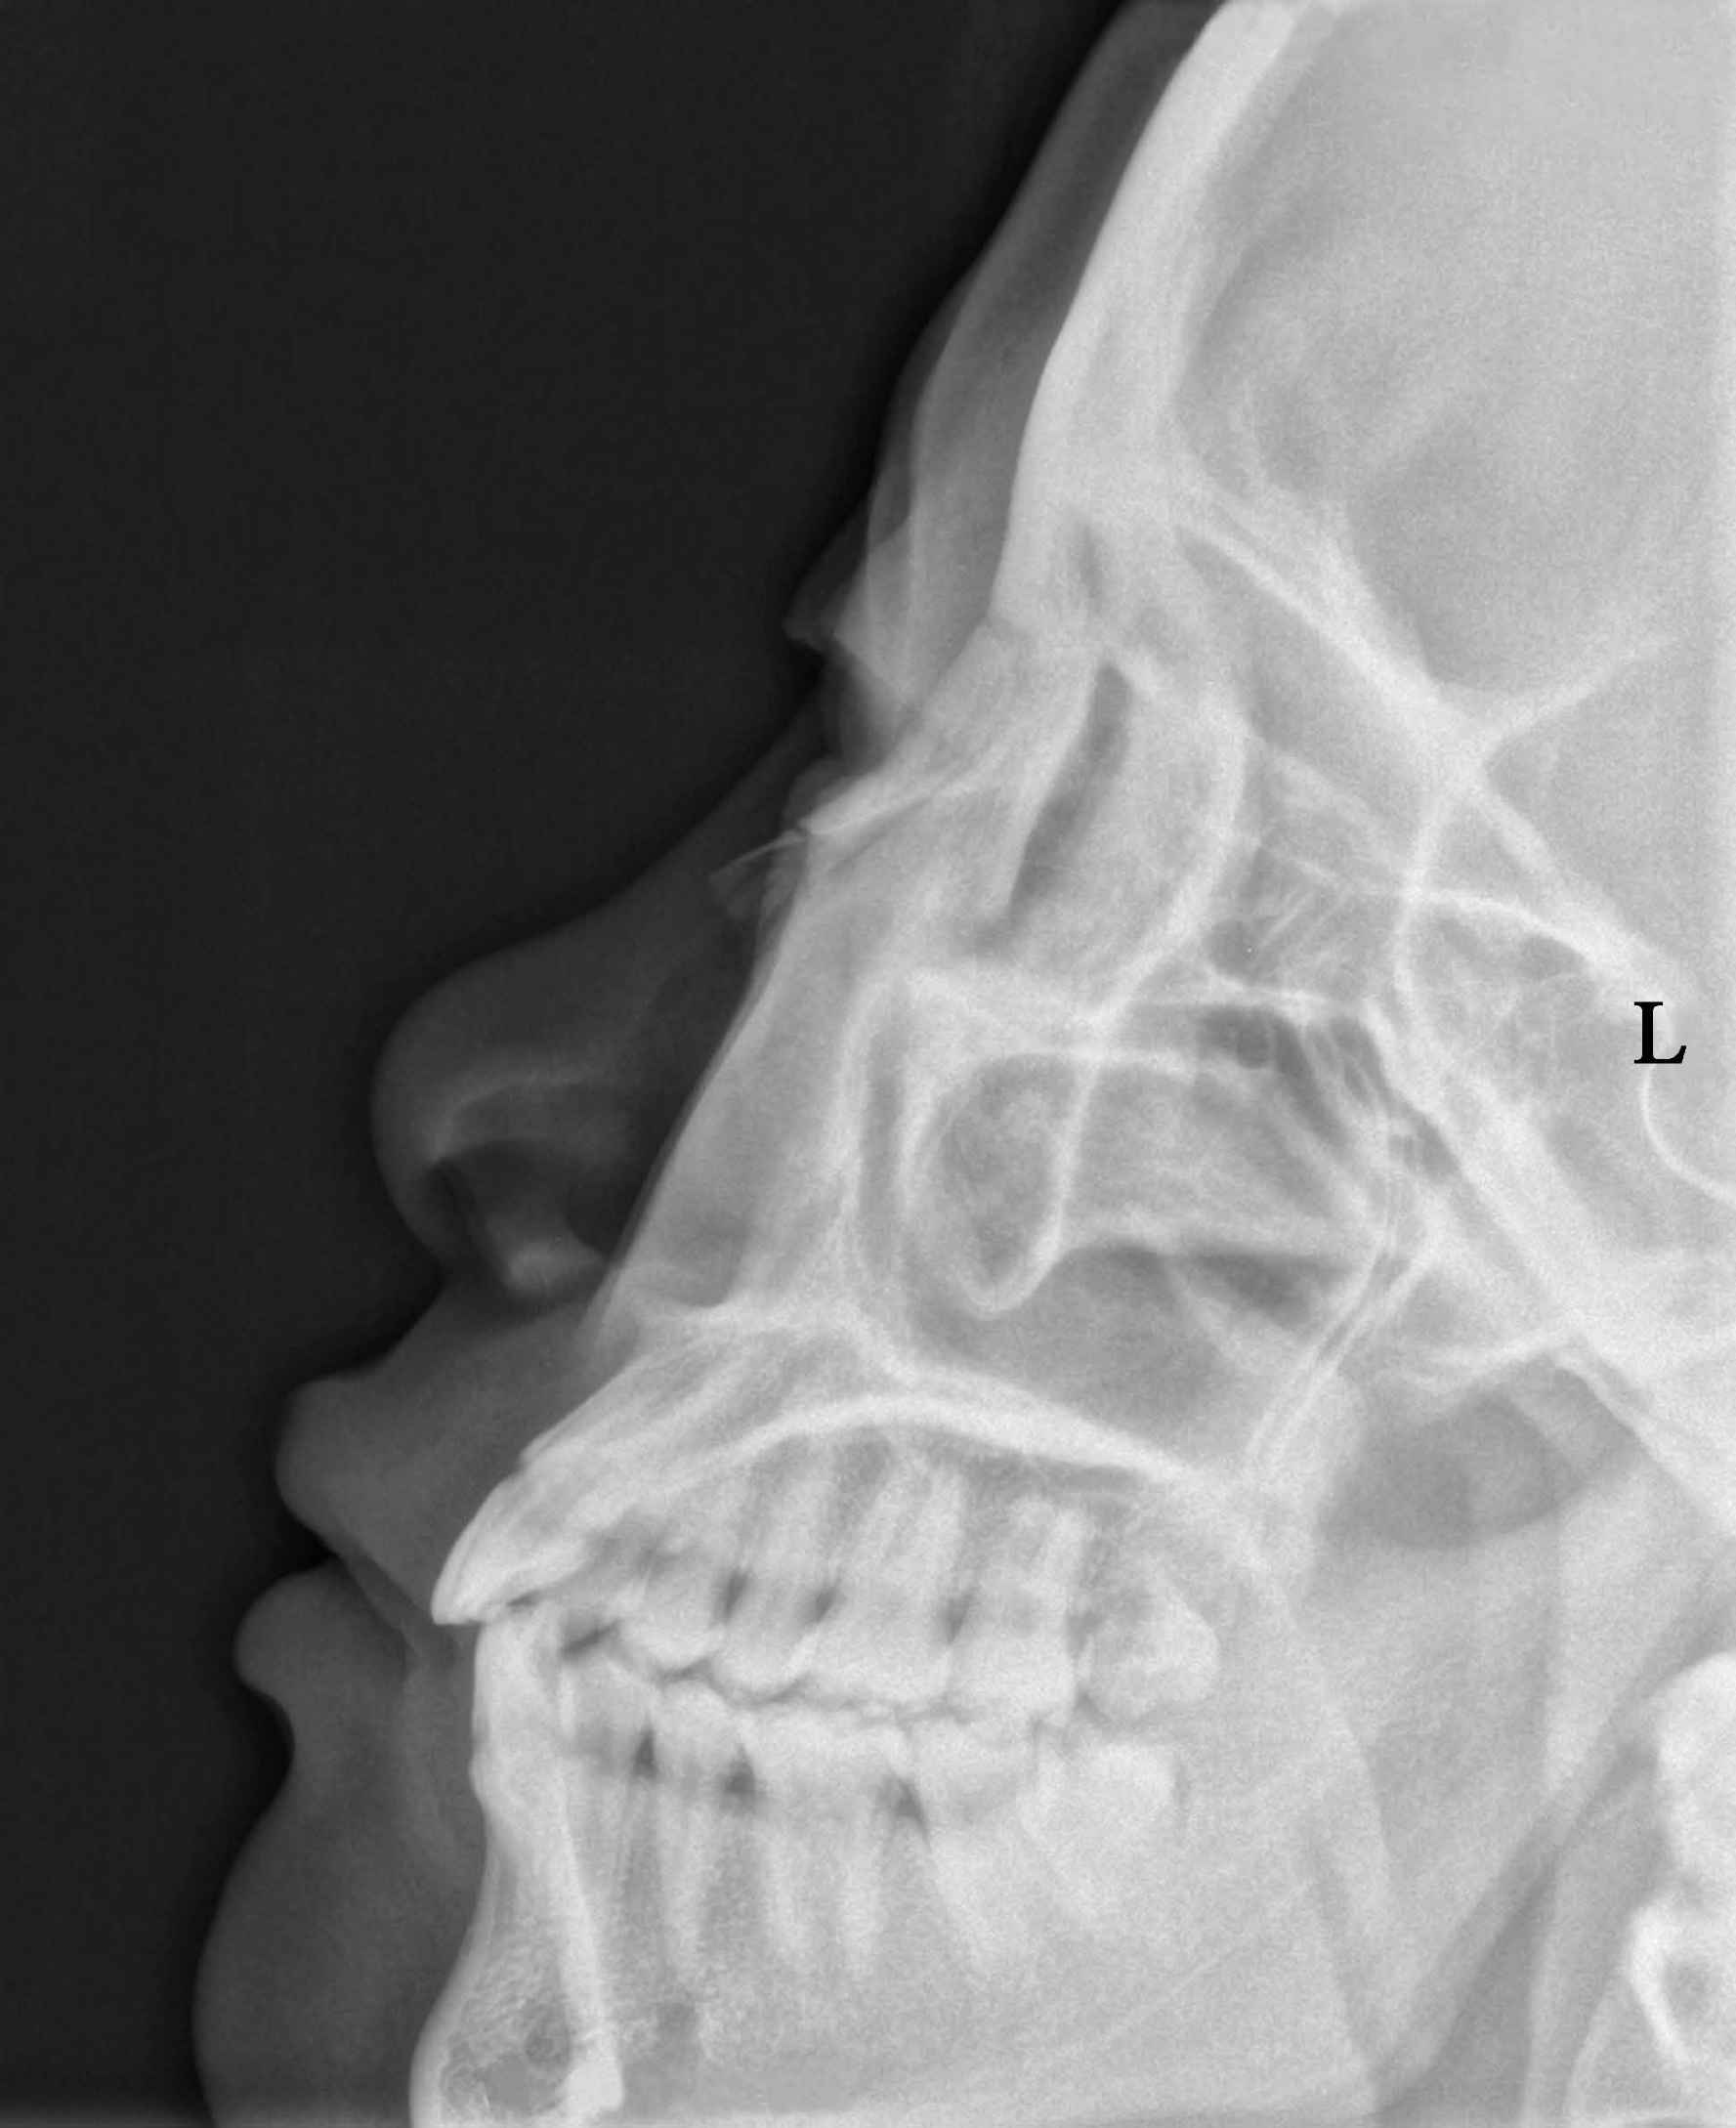
\includegraphics{./images/Image00427.jpg}
 \captionsetup{justification=centering}
 \caption{鼻骨侧位,鼻骨骨折}
 \label{fig7-4-1}
  \end{figure} 

\textbf{【病史摘要】}  男性,40岁。鼻部拳打损伤约1个小时,鼻尖部疼痛。

\textbf{【X线表现】}  鼻骨鼻尖部骨皮质不连续,局部凹陷断裂。

\textbf{【X线诊断】}  鼻骨骨折。

\textbf{【评  述】}
 本病较常见,可单发,或与颅面骨骨折并发。分为线状、移位或粉碎性骨折。侧位片可见一条横形或斜形透亮线或呈凹陷性改变,可伴有皮肤或粘膜的损伤,有时可见积气等。

\subsection{筛窦骨瘤}

\begin{figure}[!htbp]
 \centering
 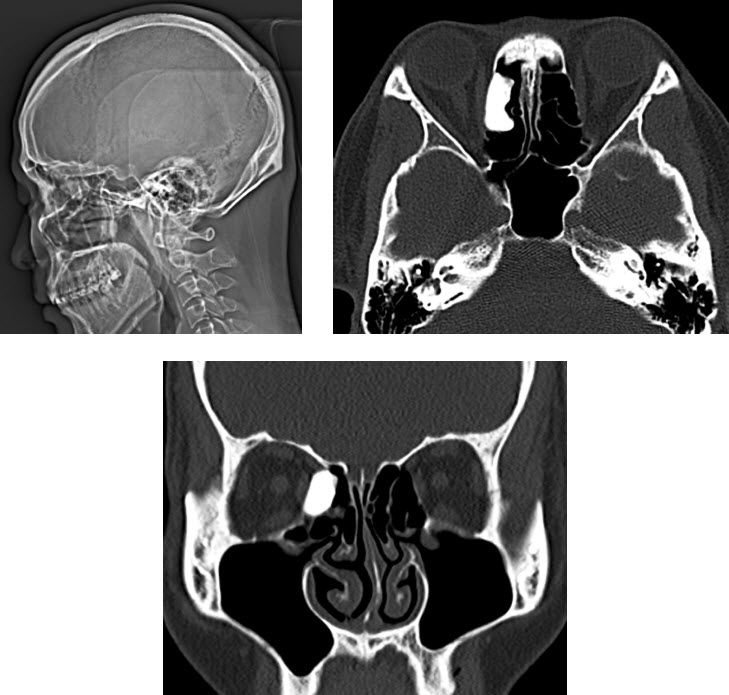
\includegraphics{./images/Image00428.jpg}
 \captionsetup{justification=centering}
 \caption{筛窦骨瘤}
 \label{fig7-4-2}
  \end{figure} 

\textbf{【病史摘要】}  男性,49岁。前额部触及骨性隆起1年余。

\textbf{【X线表现】}
 头颅侧位片示筛窦部前缘可见骨性隆起,密度与骨质密度类似。CT横断位片及冠状位片示右组筛窦内见椭圆形高密度影,密度近似骨皮质,边缘光整。

\textbf{【X线诊断】}  筛窦骨瘤(致密型)。

\textbf{【评  述】}
 骨瘤是鼻窦常见的良性肿瘤,多见于20~40岁。分为致密型、松质型和混合型。骨瘤多见于额窦,其次为筛窦、上颌窦。X线表现为圆形或卵圆形,大小不等,致密型呈高密度,类似象牙质状;松质型外围为高密度致密骨,内为松质骨,类似海绵状;混合型由两种混合构成。

\subsection{上颌窦炎}

\begin{figure}[!htbp]
 \centering
 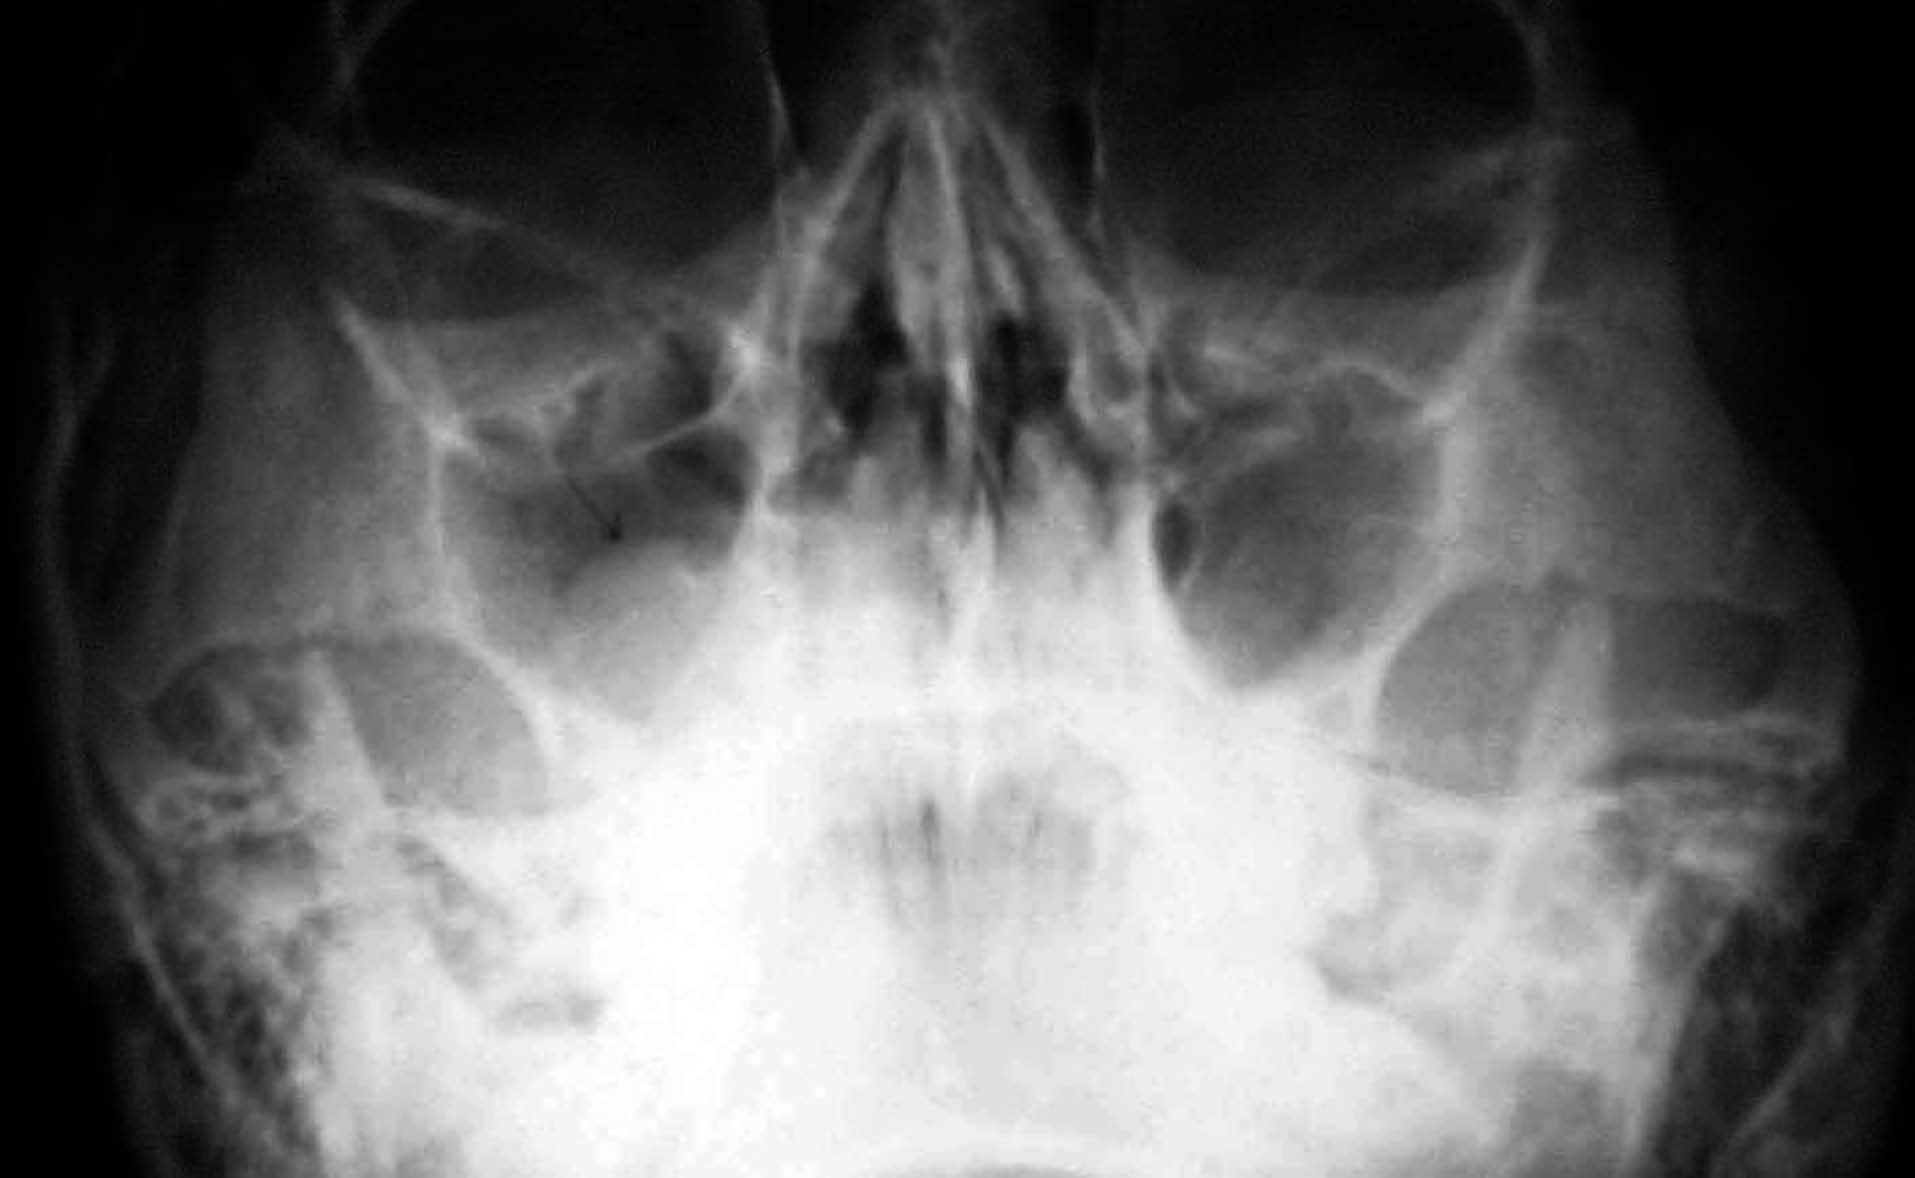
\includegraphics{./images/Image00429.jpg}
 \captionsetup{justification=centering}
 \caption{右侧上颌窦炎}
 \label{fig7-4-3}
  \end{figure} 

\textbf{【病史摘要】}  男性,56岁。流脓涕4年余,偶见血丝。

\textbf{【X线表现】}  右侧上颌窦下壁及外侧壁粘膜增厚,窦壁骨质稍变薄。

\textbf{【X线诊断】}  右侧上颌窦炎。

\textbf{【评  述】}
 鼻窦炎是鼻部最常见的病变,可继发于感染、过敏、免疫状态改变或以上几种因素共同作用。由于炎症反应,鼻窦粘膜肿胀、窦口鼻道复合体狭窄,导致粘液阻塞和分泌物潴留。鼻窦炎按病程可分为急性及慢性炎症。急性或慢性上颌窦炎均有粘膜增厚,表现为环绕窦壁的带状阴影和窦壁平行,中央有透光区,有时粘膜可高度肿胀,闭塞整个窦腔;窦内积液,于坐位水平投照为显示上颌窦积液的最好方法。慢性炎症可见窦壁硬化增白。

\subsection{鼻旁窦炎}

\begin{figure}[!htbp]
 \centering
 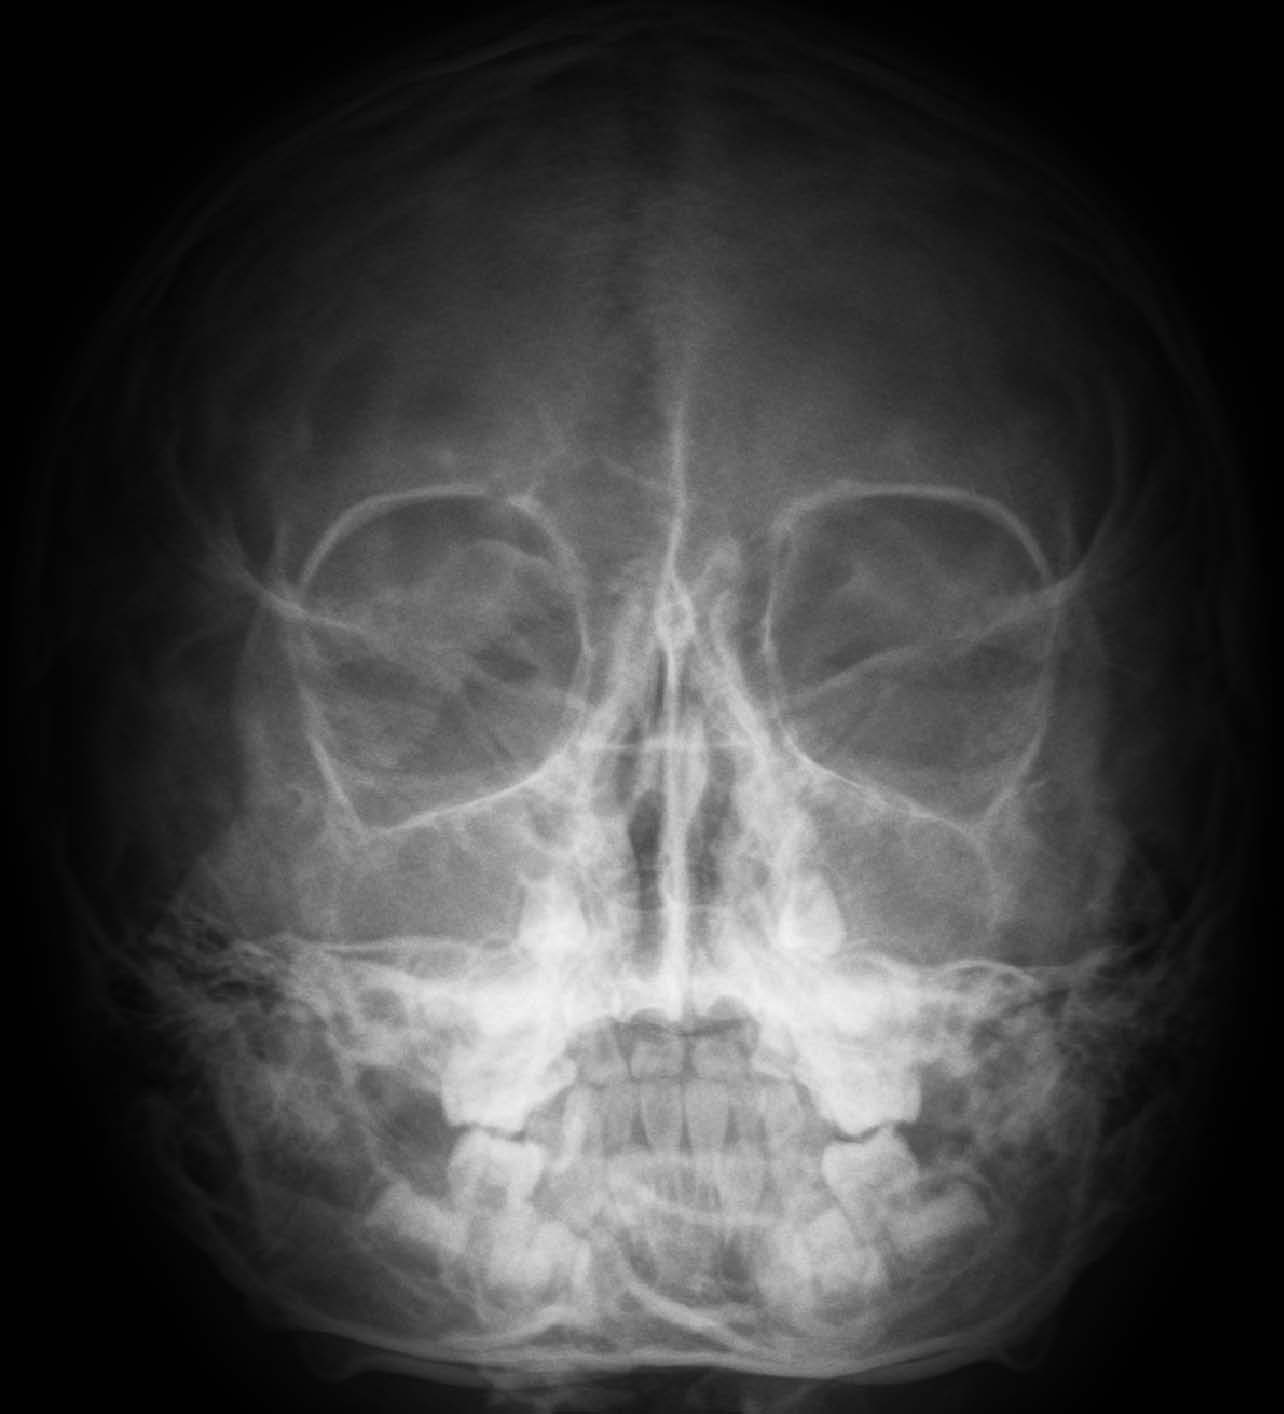
\includegraphics{./images/Image00430.jpg}
 \captionsetup{justification=centering}
 \caption{鼻旁窦炎}
 \label{fig7-4-4}
  \end{figure} 

\textbf{【病史摘要】}
 女性,8岁。发热,流脓涕2天。体格检查:双侧上颌窦区压痛。

\textbf{【X线表现】}
 双侧筛窦、额窦及上颌窦密度均增高,窦壁未见明显破坏。

\textbf{【X线诊断】}  全组鼻旁窦炎。

\textbf{【评  述】}
 鼻窦炎为常见病变,感染多来自鼻窦,少数来自咽部。上呼吸道感染,异物或外伤等是常见诱因,局部因素如鼻中隔偏曲、鼻甲肥大等也可诱发。急性鼻窦炎除有全身不适、头痛、发热等全身症状外还可有鼻窦区疼痛等,慢性鼻窦炎可无全身症状,临床常以鼻塞、流鼻涕为著。鼻窦炎的主要X线表现为鼻腔软组织增生,窦腔透亮度减低,窦腔软组织增厚,窦腔壁骨质变薄,邻近结构的侵犯。

\subsection{鼻窦粘膜囊肿}

\begin{figure}[!htbp]
 \centering
 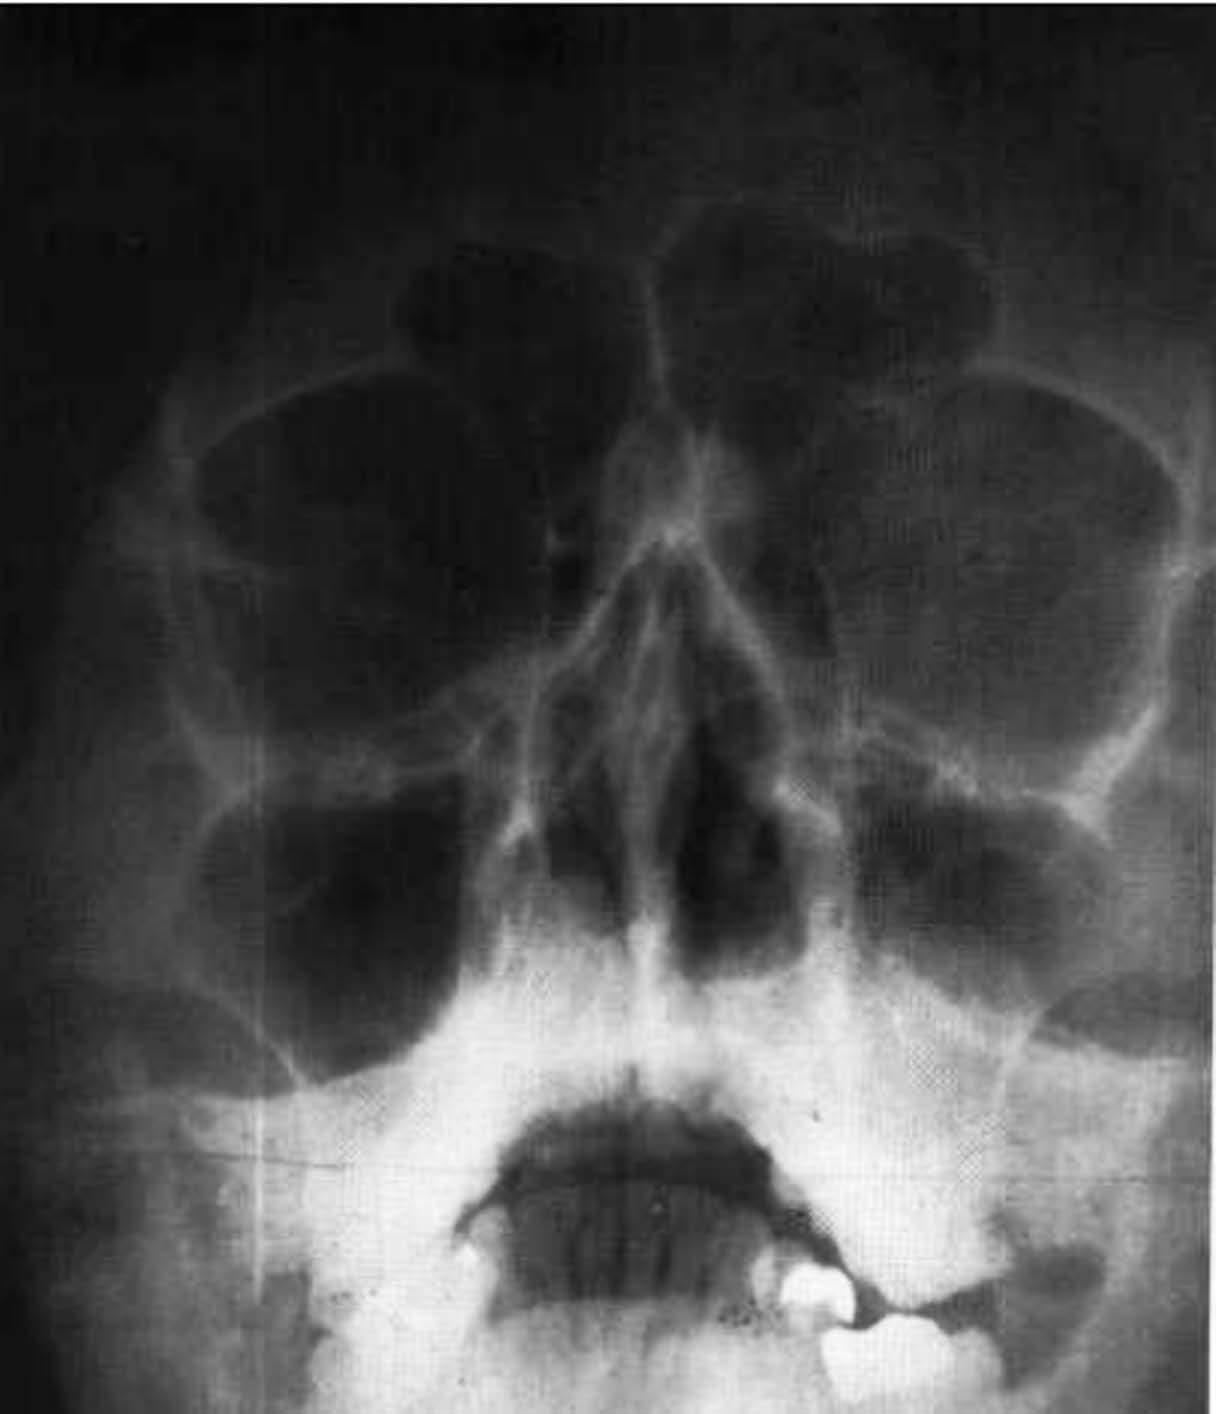
\includegraphics{./images/Image00431.jpg}
 \captionsetup{justification=centering}
 \caption{左侧上颌窦粘膜下囊肿华氏位}
 \label{fig7-4-5}
  \end{figure} 

\textbf{【病史摘要】}  男性,30岁。左鼻经常流鼻涕,近年加重。

\textbf{【X线表现】}
 左侧上颌窦底部可见一枚类圆形软组织影,密度均匀,表面光滑,周边窦壁未见明显受压。右侧上颌窦粘膜增厚。

\textbf{【X线诊断】}  左侧上颌窦粘膜囊肿,右侧上颌窦炎。

\textbf{【评  述】}
 鼻窦的粘膜囊肿主要有粘液腺潴留囊肿和粘膜下囊肿。一般无症状,多为X线检查发现。少数可自行破裂,鼻流黄水,一般不引起窦腔扩大和骨质改变。普通X线检查以华氏位显示最佳,柯氏位和侧位可辅助诊断。囊肿多见于上颌窦,沿着窦壁可见半球形软组织突入窦腔,边界较清楚,大的囊肿可充满窦腔,表现为窦腔透亮度减低,窦壁骨质一般不受累。需要鉴别诊断的是鼻窦粘液囊肿及鼻窦肿瘤。粘液囊肿更多见于额窦、筛窦,呈明显膨胀改变,易侵入邻近结构。而鼻窦肿瘤仅靠普通X线检查鉴别较难,需结合CT或MRI检查,一般肿瘤在CT或MRI上呈实性强化,而囊肿无强化。

\subsection{鼻窦粘液囊肿}

\begin{figure}[!htbp]
 \centering
 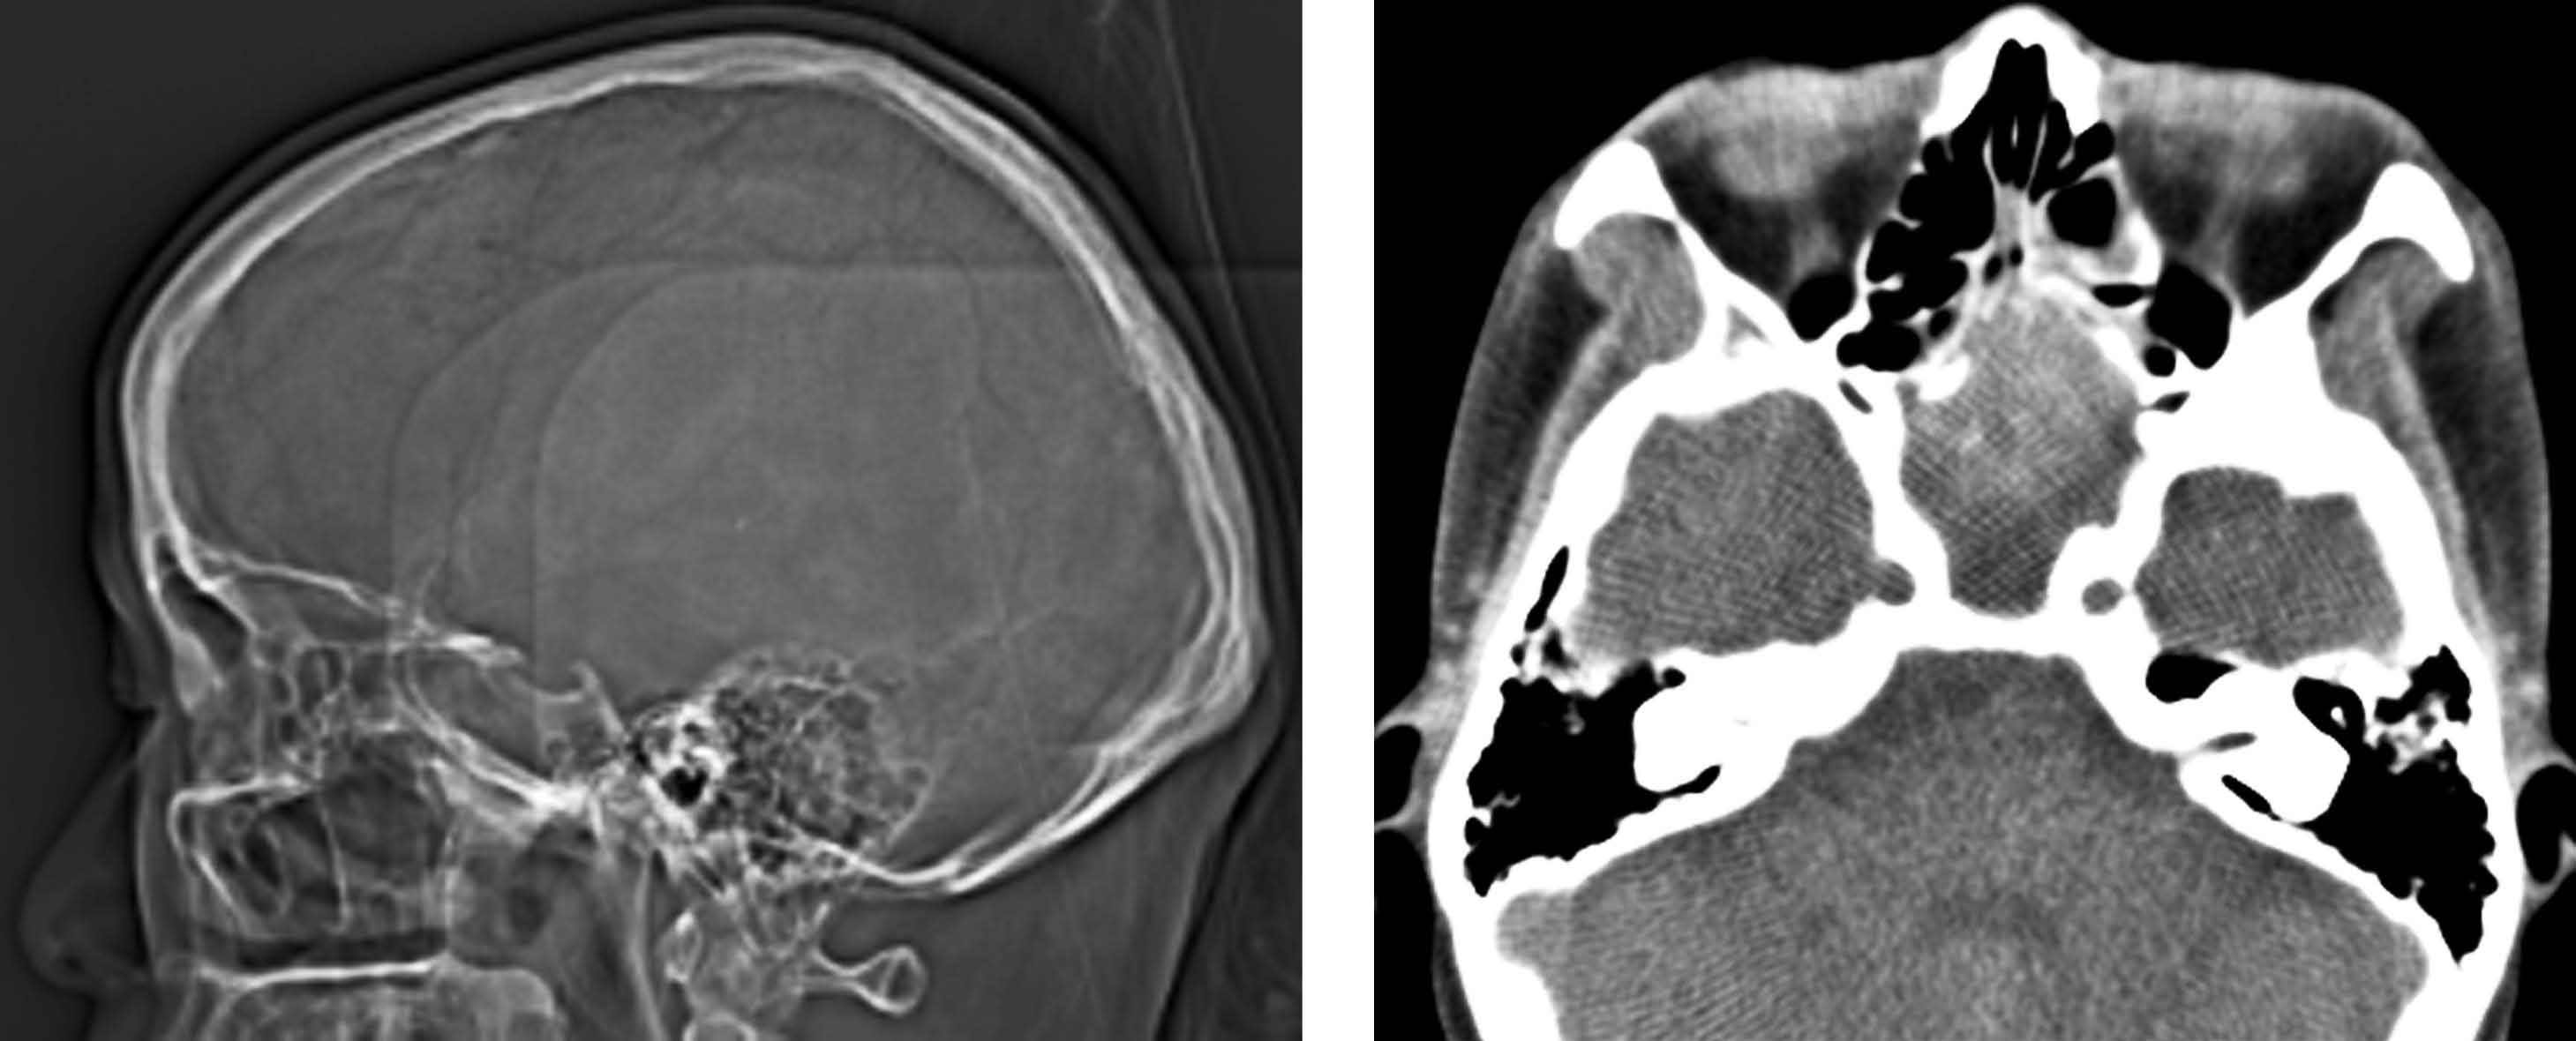
\includegraphics{./images/Image00432.jpg}
 \captionsetup{justification=centering}
 \caption{筛窦、蝶窦粘液囊肿}
 \label{fig7-4-6}
  \end{figure} 

\textbf{【病史摘要】}  女性,26岁。鼻塞、头痛数月。

\textbf{【X线表现】}
 头颅侧位片可见蝶窦区密度明显增高,蝶窦扩大。CT横断位片示蝶窦膨胀性扩大,骨壁吸收改变,蝶窦及筛窦内见软组织密度影。

\textbf{【X线诊断】}  蝶窦粘液囊肿。

\textbf{【评  述】}
 鼻窦粘液囊肿多是窦腔开口阻塞而造成窦腔膨胀性病变,通常继发于炎症。粘液囊肿壁即囊腔膜因受压变薄,纤维柱状上皮变为扁平形,粘膜下层可见炎性细胞浸润。粘液囊肿绝大多数为单发,极少数为多发。额窦最常累及,多见于中老年人,其次为筛窦,多见于青年或中年人,上颌窦及蝶窦受累较少。粘液囊肿生长缓慢,患者早期无任何不适,随着囊肿逐渐扩大,压迫囊壁而出现相应症状,额窦、筛窦粘液囊肿多因眼球突出就诊,蝶窦粘液囊肿最常见症状为视力下降,严重者可出现眶尖综合征。X线表现为窦腔透亮度改变,窦腔密度增高呈膨胀性扩大,窦壁膨隆变形,且最先向压力小的眼眶内上方移位;窦壁骨质改变,窦壁吸收变薄,窦周骨质呈硬化改变,以筛窦间隔和纸板消失最常见。鼻窦粘液囊肿病史常有典型的影像学表现,一般诊断不难。主要应与鼻窦肿瘤及粘膜下囊肿鉴别。鼻窦肿瘤CT及MRI呈均匀或不均匀的实性强化;粘膜下囊肿紧贴窦壁,一般不会引起窦壁骨质变薄、吸收,亦不会造成窦腔膨胀改变。

\subsection{上颌窦癌}

\begin{figure}[!htbp]
 \centering
 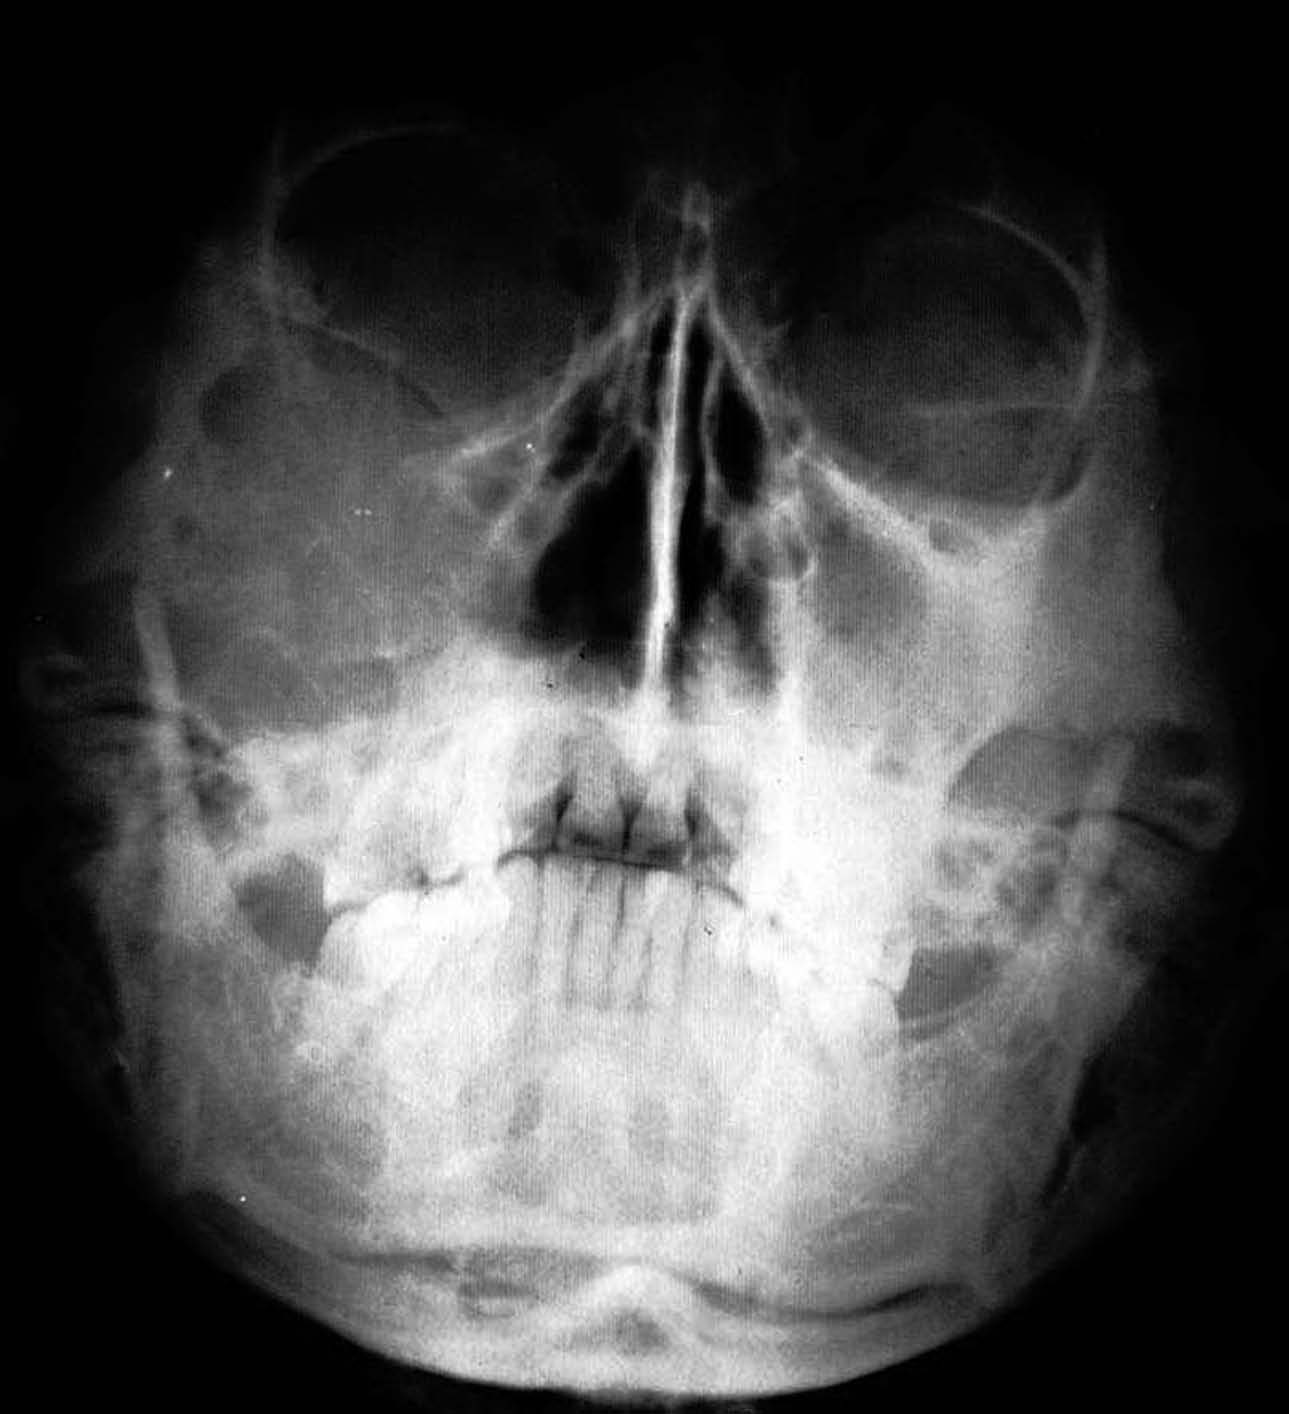
\includegraphics{./images/Image00433.jpg}
 \captionsetup{justification=centering}
 \caption{右侧上颌窦癌}
 \label{fig7-4-7}
  \end{figure} 

\textbf{【病史摘要】}  男性,68岁。右侧颌面部肿胀,疼痛4个月。

\textbf{【X线表现】}
 右侧上颌窦明显扩大,周边窦壁边界模糊,骨质破坏,向周边浸润生长,向上累及眶下缘。

\textbf{【X线诊断】}  右侧上颌窦癌。

\textbf{【评  述】}
 鼻及鼻窦恶性肿瘤较少见,大约占所有头颈部肿瘤的3%,其中最多见于上颌窦。鼻及鼻窦恶性肿瘤的早期症状与慢性鼻窦炎相似,为持续性流涕和面部疼痛,偶尔伴血涕,出现血涕应引起重视。上颌窦癌是最常见的鼻窦恶性肿瘤。主要X线表现为窦腔内软组织肿块,鼻窦透亮度减低,窦壁骨质破坏和周围软组织侵犯,少数有窦腔变大和骨质增生变化。鼻窦透亮度减低不具有特异性,鼻窦炎亦可有此种表现;骨质破坏最具特征性,对肿瘤发生部位、侵犯范围和病变性质有重要提示作用。一般早期骨质破坏程度轻,X线较难早期发现,晚期骨质破坏范围大,累及重要结构。上颌窦癌以内侧壁破坏最常见,次为眶底壁,一般向上累及筛窦;向后破坏上颌窦后外侧壁及翼腭窝,甚至可累及翼突、蝶骨大翼等;向下可累及下牙槽和硬腭;向外可致颧突破坏;晚期患者还可见眶下神经管或圆孔的破坏。CT和MRI对病变的侵犯及扩展程度有更大优势。

\section{颈部}

\subsection{咽后脓肿}

\begin{figure}[!htbp]
 \centering
 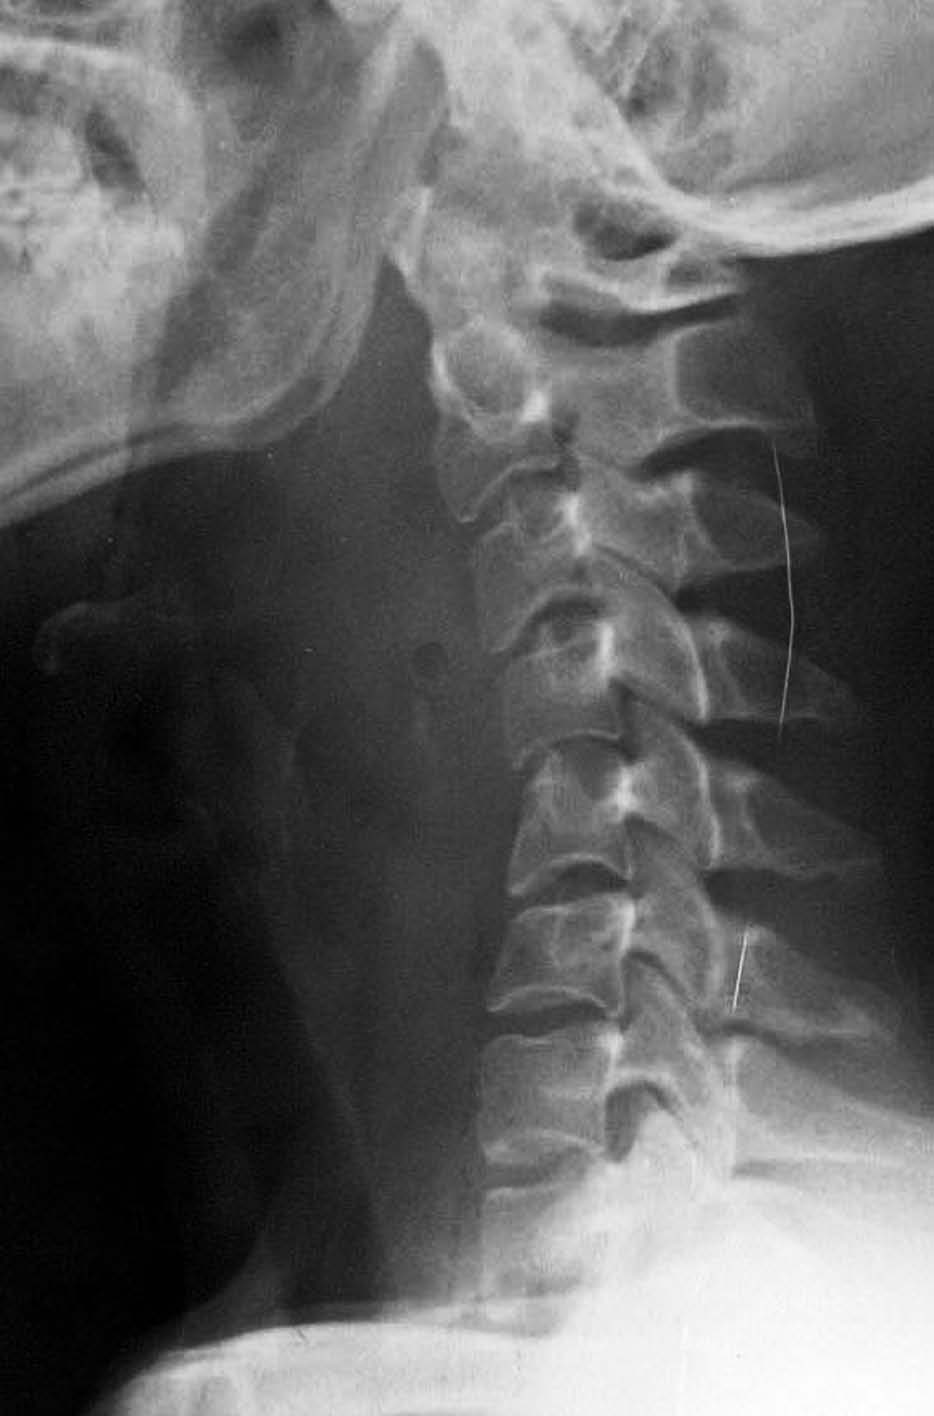
\includegraphics{./images/Image00434.jpg}
 \captionsetup{justification=centering}
 \caption{咽后壁脓肿}
 \label{fig7-5-1}
  \end{figure} 

\textbf{【病史摘要】}  女性,42岁。咽部疼痛7天,高热4天。

\textbf{【X线表现】}
 C3~T1椎体水平咽后壁软组织呈梭形肿胀,最厚处约4cm,增厚软组织中似见气泡影,颈椎受压生理曲度呈反弧表现,气管向前推移。

\textbf{【X线诊断】}  咽后壁脓肿。

\textbf{【评  述】}
 咽后壁脓肿主要来源于咽后间隙的淋巴结炎症,常见于婴幼儿,少数为咽后壁异物或损伤引起。正常人咽后壁厚度约为C4或C5椎体前后径的1/5。若超过一般表明咽后壁增厚,一般以颈部侧位片为基础,表现为软组织肿胀增厚,向前推移气管,若肿胀的软组织中间可见气体或液平则强烈提示咽后壁脓肿。软组织向后压迫颈椎,可致颈椎生理弧度改变,如消失、变直或反弧。若脓肿长期存在可致椎体骨质改变,还可引起椎前韧带的骨化或钙化。咽后脓肿表现为咽后壁软组织增厚,但缺乏特异性,血肿、肉芽肿及恶性淋巴瘤等也有这种表现。

\subsection{腺样体肥大}

\begin{figure}[!htbp]
 \centering
 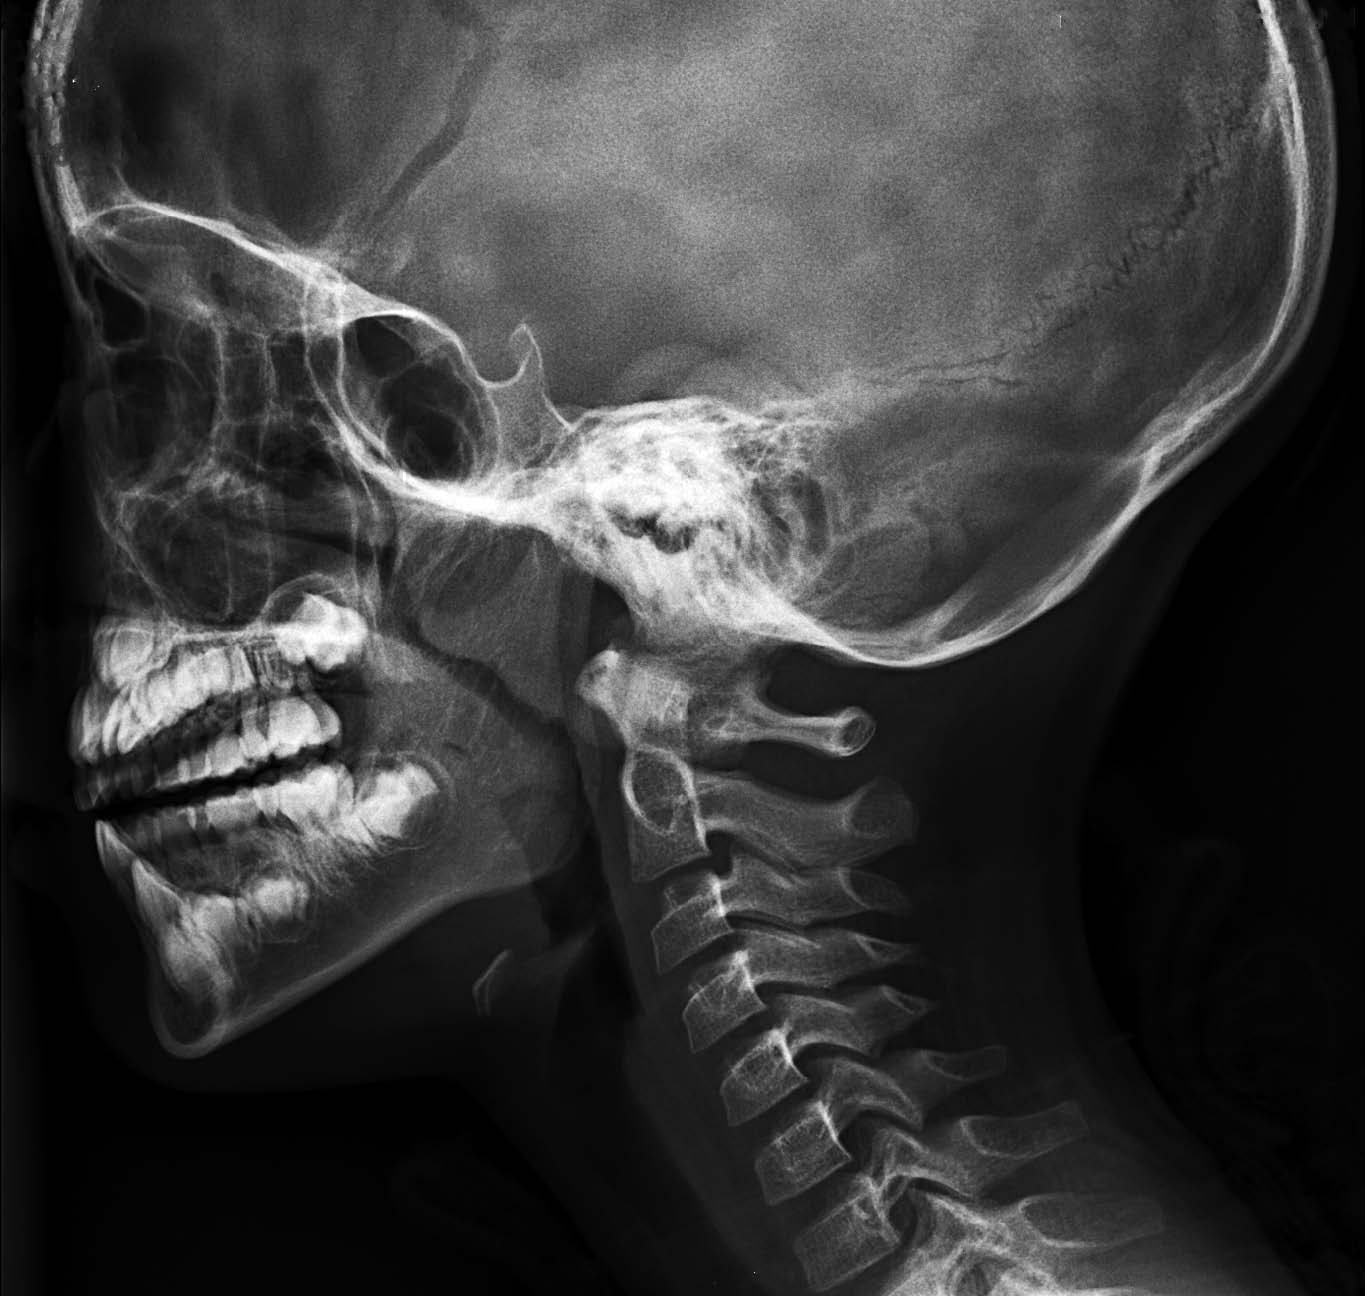
\includegraphics{./images/Image00435.jpg}
 \captionsetup{justification=centering}
 \caption{腺样体肥大}
 \label{fig7-5-2}
  \end{figure} 

\textbf{【病史摘要】}  男性,7岁。夜间打鼾1个月余。

\textbf{【X线表现】}
 鼻咽腔后顶部软组织增厚,向前压迫气道,气道轻度变窄,于第2颈椎水平狭窄约1/3以下。

\textbf{【X线诊断】}  腺样体轻度肥大。

\textbf{【评  述】}
 小儿腺样体肥大或增生是小儿打鼾的主要原因,腺样体肥大可引起鼻咽腔气道狭窄。判断腺样体增生程度主要测量鼻咽腔顶后壁软组织影的厚度,根据气道狭窄程度分三度,轻度、中度、重度。具体方法:在侧位片上,以第2颈椎上缘水平处的气道为基准,气道受压在1/3以下为轻度,2/3以下为中度,2/3以上为重度。颈部侧位片可较清楚显示腺样体增大的部位和局部气道狭窄的程度,可以辅助制订手术计划。

\subsection{鼻咽癌}

\begin{figure}[!htbp]
 \centering
 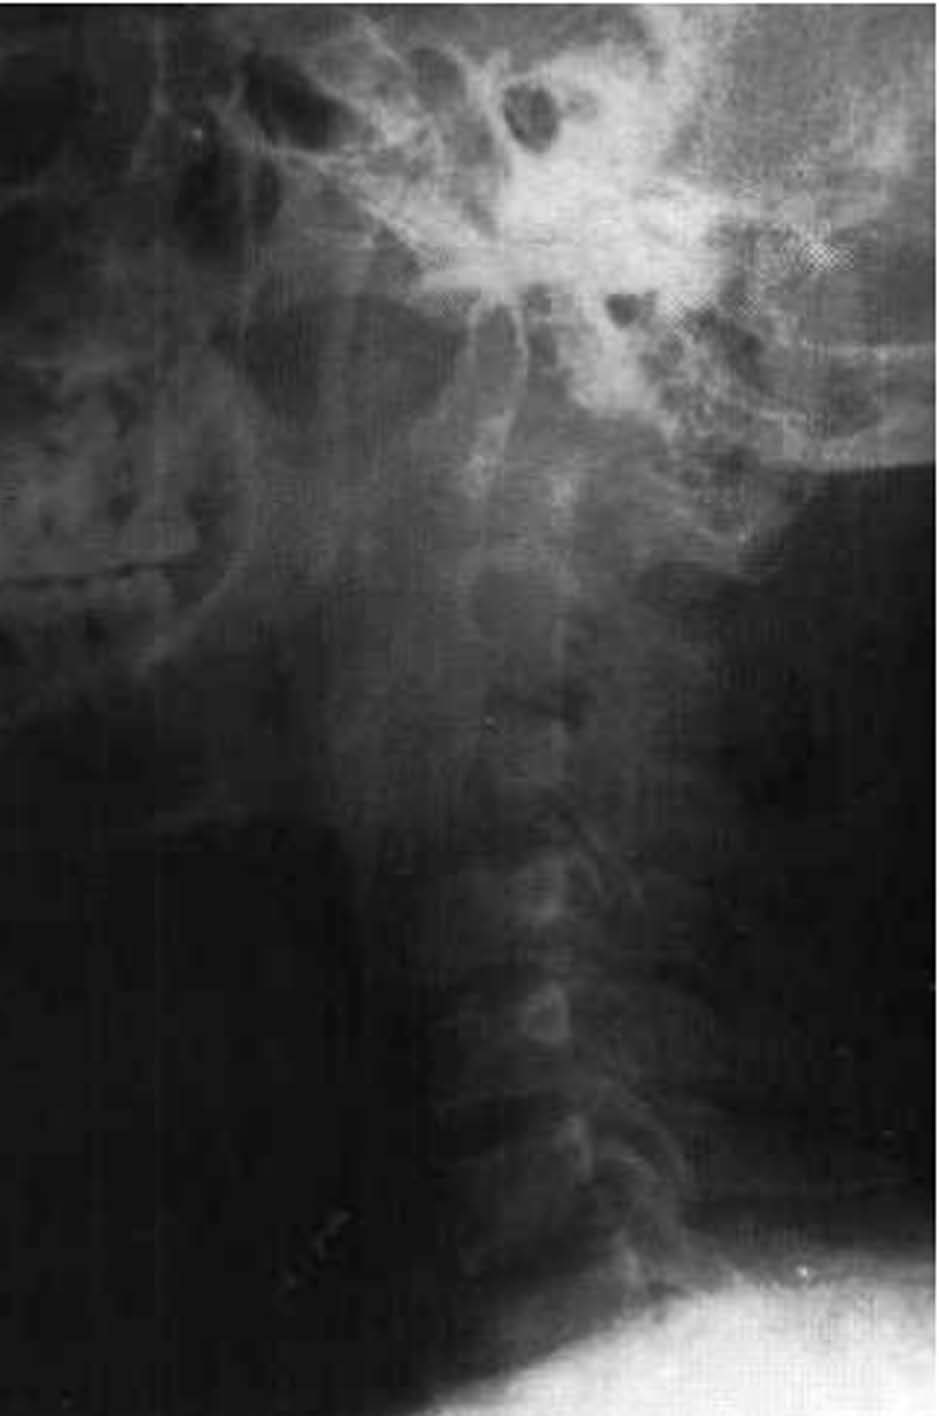
\includegraphics{./images/Image00436.jpg}
 \captionsetup{justification=centering}
 \caption{颈部侧位片(鼻咽癌)}
 \label{fig7-5-3}
  \end{figure} 

\textbf{【病史摘要】}
 女性,45岁。发现颈部肿块1天入院。体格检查:左侧颈部触及直径约3cm左右包块。

\textbf{【X线表现】}
 鼻咽部顶后壁软组织增厚、肿胀,向前隆起。颈椎椎体未见明显骨质破坏。

\textbf{【X线诊断】}  鼻咽癌。

\textbf{【评  述】}
 鼻咽癌是发生于鼻咽部上皮细胞的恶性肿瘤,大多数鼻咽癌起自咽隐窝。早期鼻咽癌的临床表现常较隐匿,中、晚期鼻咽癌因肿物的侵犯范围不同而表现各异。患者就诊时往往以颈部淋巴结肿大为首发症状,其主要临床症状有回缩性血涕、鼻出血等。鼻咽癌X线检查常规应该摄取鼻咽侧位片及颅底片。主要X线表现为鼻咽部软组织肿块,癌肿向上可侵蚀颅底骨质,表现为骨质破坏,少数为骨质硬化。鼻咽癌需与鼻咽部病变如鼻咽部纤维血管瘤鉴别。鼻咽部纤维血管瘤也可引起骨质改变呈压迫性吸收、变形,但临床多见于青年男性,有反复多量出血史,这有助于两者鉴别。

